\documentclass[]{article}
\usepackage{lmodern}
\usepackage{amssymb,amsmath}
\usepackage{ifxetex,ifluatex}
\usepackage{fixltx2e} % provides \textsubscript
\ifnum 0\ifxetex 1\fi\ifluatex 1\fi=0 % if pdftex
  \usepackage[T1]{fontenc}
  \usepackage[utf8]{inputenc}
\else % if luatex or xelatex
  \ifxetex
    \usepackage{mathspec}
  \else
    \usepackage{fontspec}
  \fi
  \defaultfontfeatures{Ligatures=TeX,Scale=MatchLowercase}
\fi
% use upquote if available, for straight quotes in verbatim environments
\IfFileExists{upquote.sty}{\usepackage{upquote}}{}
% use microtype if available
\IfFileExists{microtype.sty}{%
\usepackage{microtype}
\UseMicrotypeSet[protrusion]{basicmath} % disable protrusion for tt fonts
}{}
\usepackage[margin=1.5in]{geometry}
\usepackage{hyperref}
\hypersetup{unicode=true,
            pdftitle={Factors Influencing Inference of Clonality in Diploid Populations},
            pdfauthor={Zhian N. Kamvar; Niklaus J. Grünwald},
            pdfborder={0 0 0},
            breaklinks=true}
\urlstyle{same}  % don't use monospace font for urls
\usepackage{longtable,booktabs}
\usepackage{graphicx,grffile}
\makeatletter
\def\maxwidth{\ifdim\Gin@nat@width>\linewidth\linewidth\else\Gin@nat@width\fi}
\def\maxheight{\ifdim\Gin@nat@height>\textheight\textheight\else\Gin@nat@height\fi}
\makeatother
% Scale images if necessary, so that they will not overflow the page
% margins by default, and it is still possible to overwrite the defaults
% using explicit options in \includegraphics[width, height, ...]{}
\setkeys{Gin}{width=\maxwidth,height=\maxheight,keepaspectratio}
\IfFileExists{parskip.sty}{%
\usepackage{parskip}
}{% else
\setlength{\parindent}{0pt}
\setlength{\parskip}{6pt plus 2pt minus 1pt}
}
\setlength{\emergencystretch}{3em}  % prevent overfull lines
\providecommand{\tightlist}{%
  \setlength{\itemsep}{0pt}\setlength{\parskip}{0pt}}
\setcounter{secnumdepth}{5}
% Redefines (sub)paragraphs to behave more like sections
\ifx\paragraph\undefined\else
\let\oldparagraph\paragraph
\renewcommand{\paragraph}[1]{\oldparagraph{#1}\mbox{}}
\fi
\ifx\subparagraph\undefined\else
\let\oldsubparagraph\subparagraph
\renewcommand{\subparagraph}[1]{\oldsubparagraph{#1}\mbox{}}
\fi

%%% Use protect on footnotes to avoid problems with footnotes in titles
\let\rmarkdownfootnote\footnote%
\def\footnote{\protect\rmarkdownfootnote}

%%% Change title format to be more compact
\usepackage{titling}

% Create subtitle command for use in maketitle
\newcommand{\subtitle}[1]{
  \posttitle{
    \begin{center}\large#1\end{center}
    }
}

\setlength{\droptitle}{-2em}
  \title{Factors Influencing Inference of Clonality in Diploid Populations}
  \pretitle{\vspace{\droptitle}\centering\huge}
  \posttitle{\par}
  \author{Zhian N. Kamvar \\ Niklaus J. Grünwald}
  \preauthor{\centering\large\emph}
  \postauthor{\par}
  \predate{\centering\large\emph}
  \postdate{\par}
  \date{2017-07-16}


\usepackage{amsthm}
\newtheorem{theorem}{Theorem}[section]
\newtheorem{lemma}{Lemma}[section]
\theoremstyle{definition}
\newtheorem{definition}{Definition}[section]
\newtheorem{corollary}{Corollary}[section]
\newtheorem{proposition}{Proposition}[section]
\theoremstyle{definition}
\newtheorem{example}{Example}[section]
\theoremstyle{remark}
\newtheorem*{remark}{Remark}
\begin{document}
\maketitle
\begin{abstract}
The index of association is a measure of multilocus linkage
disequilibrium that reflects the deviation of observed genetic variation
from expected. In sexual populations, loci are randomly assorting due to
recombination, resulting in a near-zero value of the index of
association. In clonal populations, recombination is non-existent,
meaning that loci are passed from parent to offspring in a
non-independent fashion, resulting in a significantly non-zero value of
the index of association. We build on previous work by investigating the
effect of sample size, mutation rate, and clone correction on the power
of the index of association to detect clonal reproduction in simulated
data sets generated with microsatellite and genomic markers. Our
findings suggest that power decreases with small sample sizes and low
allelic diversity. Additionally, we find that physical linkage in
genomic markers does not affect power if permutation tests are performed
with linkage groups. We hope that these novel insights provide useful to
the study of molecular pathogens.
\end{abstract}

\section{Introduction}\label{introduction}

Population genetic theory is largely based on model populations such as
the neutral Wright-Fisher model in which populations are assumed to be
infinitely large, with discrete generations, randomly assorting alleles,
with no migration and no mutation (Hartl \& Clark 2007; Nielsen \&
Slatkin 2013). By using such reductionist models, population geneticists
are able to reduce the complexity and enable analyses to ask fundamental
questions and test hypotheses about evolutionary processes that could
explain population structure and history.

These neutral models, however, cannot be applied to populations whose
life history violate the fundamental assumption of random assortment of
alleles, such as populations that undergo clonal reproduction (Orive
1993; Milgroom 1996). For many clonal populations, the contribution of
genetic variation from mutation is greater than that of recombination.
While this increases the risk of deleterious mutation accumulation,
selectively advantageous combinations of alleles are maintained (Heitman
\emph{et al.} 2012).

Pathogenic microorganisms can reproduce sexually or clonally (Milgroom
1996; Tibayrenc 1996). Diseases caused by these organisms are in part
managed by the use of antimicrobial compounds that kill these organisms.
Detecting recombination in populations of pathogenic microorganisms is
therefore important for the implementation of rational management
strategies as a prevalence of sexual reproduction could lead to the
repeated emergence of novel, resistant genotypes (Smith \emph{et al.}
1993; Milgroom 1996; de Meeûs \emph{et al.} 2006; Goss \emph{et al.}
2014; Nieuwenhuis \& James 2016).

Several studies have attempted to infer the degree of sex in populations
that undergo clonal reproduction (Smith \emph{et al.} 1993; Balloux
\emph{et al.} 2003; de Meeûs \& Balloux 2004; Ali \emph{et al.} 2016;
Nieuwenhuis \& James 2016). For populations with well-defined sexual and
clonal phases occurring at separate times, such as rust fungi, methods
like \emph{CloNcaSe} are effective for estimating the rate of sexual
reproduction and effective population size (Ali \emph{et al.} 2016).
However, this method cannot be applied to populations where the
reproductive cycle is not partitioned into discrete generations.

Simply detecting the presence of clonal reproduction, however can be
useful in and of itself (Milgroom 1996). A method commonly used to
assess this is the index of association (\(I_A\)), and its standardized
version, \(\bar{r}_d\), which measure multilocus linkage disequilibrium
(Brown \emph{et al.} 1980; Smith \emph{et al.} 1993; Haubold \emph{et
al.} 1998; Agapow \& Burt 2001; de Meeûs \& Balloux 2004; Kamvar
\emph{et al.} 2014). The value of \(I_A\), as shown in equation
\eqref{eq:ia}, is measured as the ratio of observed variance (\(V_O\)) and
expected variance (\(V_E\)) in genetic distance between samples (Smith
\emph{et al.} 1993; Agapow \& Burt 2001):

\begin{equation}
I_A = \frac{V_O}{V_E} - 1 \label{eq:ia}
\end{equation}

The expected variance is practically modeled as the sum of the variances
over \emph{m} loci: \(V_E = \sum^m{var_j}\) (Haubold \emph{et al.} 1998;
Agapow \& Burt 2001). If the differences between samples are randomly
distributed (linkage equilibrium), we can expect the value of \(I_A\) to
be zero (Smith \emph{et al.} 1993; Agapow \& Burt 2001). Under scenarios
of non-random mating (e.g.~population structure or clonal reproduction),
the observed variance would be greater than the expected variance due to
a multi-modal distribution of distances, and \(I_A\) would be greater
than zero (Smith \emph{et al.} 1993; Agapow \& Burt 2001; Milgroom
2015). Agapow \& Burt (2001) noted that this metric does not have an
upper limit and increases with the number of loci. To correct this, they
developed \(\bar{r}_d\) (equation \eqref{eq:rd}), which has a similar
structure to a correlation coefficient and ranges from 0 (no linkage) to
1 (complete linkage):

\begin{align} % This mode aligns the equations to the '&=' signs
\begin{split} % This mode groups the equations into one.
\bar{r}_d &= \frac{\sum\sum{cov_{j,k}}}{
                   \sum\sum{\sqrt{var_{j} \cdot var_{k}}}} \\
          &= \frac{V_O - V_E}{2\sum\sum{\sqrt{var_{j} \cdot var_{k}}}}
\end{split}
\label{eq:rd}
\end{align}

Previous research has already contributed to our understanding of the
behavior of \(\bar{r}_d\). De Meeûx \& Balloux (2004) investigated the
effect of increasing levels of sexual reproduction on \(\bar{r}_d\)
(noted in their publication as \(\bar{r}_D\)). They found that very
little (\(\sim\) 1\%) sexual reproduction is required to produce a value
of \(\bar{r}_d\) that is not significantly different from zero. This
work indicated that \(\bar{r}_d\) alone might not be well suited as a
measure of clonal reproduction. Additionally, Prugnolle \& de Meeûs
(2010) tested the effect of sampling design on \(\bar{r}_d\), finding
that its value was drastically reduced when clones from multiple
populations were sampled, leading to an over-estimation of the level of
recombination.

These studies laid the groundwork for understanding the behavior of
\(\bar{r}_d\) under different scenarios of non-random mating in diploid
organisms, but there were some limitations in available technology. For
both studies, the only software available for calculation of
\(\bar{r}_d\) for diploid organisms was \textsc{Multilocus}, which could
only take one data set at a time (Agapow \& Burt 2001; de Meeûs \&
Balloux 2004; Prugnolle \& de Meeûs 2010; Kamvar \emph{et al.} 2014).
This constrained researchers to only analyze a minimal set of 20
populations per scenario.

Furthermore, a non-zero value of \(I_A\) and \(\bar{r}_d\) does not
always indicate a significant departure from the null assumption of
unlinked loci. Since the distribution of \(I_A\) and \(\bar{r}_d\) are
not known, the safest way to test for significance are random
permutation tests. These tests effectively create unlinked populations
by shuffling individuals at each locus, independently and re-calculating
\(I_A\) and \(\bar{r}_d\) (Smith \emph{et al.} 1993; Haubold \emph{et
al.} 1998; Agapow \& Burt 2001). An upper one-sided test of significance
is then used to see if the observed statistic is greater than the
observed distribution.

Standard practice for analyzing microbial populations is to perform this
test on both the whole data set (wd) and clone-corrected data (cc),
where each multilocus genotype is represented only once per population
to avoid signatures of linkage that arise from re-sampling the same
individual (Milgroom 1996; McDonald 1997; Goss \emph{et al.} 2014). If
the p-value for \(\bar{r}_d\) is significant after clone-correction,
then the population is expected to be clonal. While significance testing
is available in \textsc{Multilocus} in the form of random permutations,
it is computationally expensive, and can only take one data set at a
time (Agapow \& Burt 2001; Kamvar \emph{et al.} 2014). As a result,
power analysis of \(\bar{r}_d\) to detect clonal reproduction with and
without clone-correction has not yet been performed (de Meeûs \& Balloux
2004).

In the years since the studies conducted by de Meeûs \& Balloux (2004)
and Prugnolle \& de Meeûs (2010), reduced-representation,
high-throughput sequencing methods such as Genotyping-By-Sequencing
(GBS) and Restriction site associated DNA sequencing (RAD-seq) have
become popular tools for population genetic analysis (Davey \& Blaxter
2010; Elshire \emph{et al.} 2011; Davey \emph{et al.} 2011). These
methods have the capability to generate thousands of unlinked markers at
a fraction of the cost and time necessary to develop high quality
microsatellite markers. These marker systems are also prone to missing
data and high error rates (Mastretta-Yanes \emph{et al.} 2014). Sentence
or two about the utility of these markers compared to SSRs for highly
clonal organisms, citing (Rafiei \emph{et al.}). The index of
association was developed for multiple loci at a time when obtaining
even 100 unlinked markers posed a significant challenge. With the advent
of these technologies, it is unclear how marker choice and genotyping
error affect the index of association.

We developed the R package \emph{poppr} for analysis of clonal
populations, removing the limitations of data input and computational
expense of analyzing the index of association (Kamvar \emph{et al.}
2014) and further expanded this to analysis of genome-wide SNP data
(Kamvar \emph{et al.} 2015a; R Core Team 2016). With these tools we
expand on previous studies by asking how sample size, marker choice,
clone-correction, and the assumption of homogeneous mutation rates
affect our ability to detect clonal reproduction in diploid populations.
Our objectives to answer these questions are to (1) re-analyze
\(\bar{r}_d\) against increasing rates of sexual reproduction in both
microsatellite and SNP data sets, (2) perform a power analysis of
\(\bar{r}_d\) to assess sensitivity and specificity, and (3) assess how
genotypic and allelic evenness and diversity affects \(\bar{r}_d\).
Because studies have observed significantly negative values of \(I_A\)
and \(\bar{r}_d\) (p \(\geq\) 0.95), we additionally seek to determine
what factors result in negative \(\bar{r}_d\) values. This work provides
novel insights into the sensitivity and scope of the index of
association for inferring clonality.

\section{Methods}\label{methods}

We used simulations to evaluate the behavior of \(\bar{r}_d\) under
different population scenarios. Initial sets of simulations were created
for different levels of sexual reproduction for each marker type. All
simulations were performed with the python package simuPOP version 1.1.7
in python version 3.4 (Peng \& Amos 2008). For each scenario, 100
simulations with 10 replicates were created with a census size of 10,000
diploid individuals (to minimize the effect of drift) with equal mating
type proportions evolved over 10,000 generations (previously shown in de
Meeûs \& Balloux (2004) to be sufficient in reaching equilibrium for
summary statistics).

The simulated populations were first stored in the native simuPOP format
and then transferred to feather format using the python and R packages
\emph{feather} version 0.3.0 for downstream analyses. Microsatellite
simulations were performed on Ubuntu Linux version 14.04; SNP
simulations were performed on CentOS Linux version 6.8. During
downstream analysis, 10, 25, 50, and 100 individuals were sampled
without replacement for each replicate in R version 3.2 with the package
\emph{poppr} version 2.3.0 (Kamvar \emph{et al.} 2014, 2015a; R Core
Team 2016). Analyses (described below) were performed on both full and
clone-corrected data sets. All downstream analyses were run on the OSU
CGRB Core Computing Facility.

\subsection{Simulating Microsatellite
Loci}\label{simulating-microsatellite-loci}

Each population was simulated with 21 co-dominant, unlinked loci
containing 6 to 10 alleles per locus with frequencies drawn from a
uniform distribution and subsequently normalized so that allele
frequencies at each locus sum to one. We used 6 to 10 alleles per locus
as this is the number of alleles commonly used for population genetic
studies to avoid statistical noise. Before mating, mutations occurred at
each locus at a rate of 1e-5 mutations/generation with the exception of
the first locus, at which the mutation rate was set to 1e-3. The
mutation rate of 1e-5 was selected as this was previously used in de
Meeûs \& Balloux (2004) and is close to the estimated recombination rate
of \emph{Saccharomyces cerevisiae} microsatellite loci (Lynch \emph{et
al.} 2008). All mutations were applied in a stepwise manner using the
\texttt{StepwiseMutator()} operator in simuPOP.

\subsection{Simulating SNP Loci}\label{simulating-snp-loci}

Simulations of 10,000 diploid, biallelic loci spread evenly over 10
chromosomal fragments were simulated with a mutation rate of 1e-5
mutations per generation for forward and backward mutations using the
\texttt{SNPMutator()} operator and and a recombination rate of 0.01
between adjacent loci using the \texttt{Recombinator()} operator in
simuPOP.

\subsection{Mating}\label{mating}

Simulations of sexual reproduction were conducted at 10 rates of sexual
reproduction over a log scale (0.0, 1e-4, 5e-4, 1e-3, 5e-3, 1e-2, 5e-2,
0.1, 0.5, 1.0) reflecting the fraction of individuals in generation
\emph{t+1} produced via sexual reproduction. One to three offspring
could be produced at each mating event. Rates were chosen to investigate
the dynamics of \(\bar{r}_d\) at low levels of clonal reproduction. For
sexual events, two parents were chosen randomly from the population with
the \texttt{RandomSelection()} operator and offspring genotypes were
created via the \texttt{MendelianGenoTransmitter()} operator. The clonal
fraction was created by randomly sampling individuals from the
population and duplicating their genotypes with the
\texttt{CloneGenoTransmitter()} operator. If one mating type was lost
before 10,000 generations, the simulation would continue to completion
with only clonal reproduction.

\subsection{Analysis of Microsatellite
Data}\label{analysis-of-microsatellite-data}

The standardized index of association (\(\bar{r}_d\), Agapow \& Burt
(2001)) was calculated for full and clone-corrected data using the
\emph{poppr} function \texttt{ia()} (Kamvar \emph{et al.} 2014). Tests
for significance were performed by randomly permuting the alleles at
each locus independently and then assessing \(\bar{r}_d\). A total of
999 permutations were conducted for each replicate population to
evaluate statistical support. Analyses were done for both full and
clone-corrected data. The p-values reflect the proportion of
observations greater than the observed statistic. Estimates of genotypic
diversity were assessed with the \emph{poppr} function
\texttt{diversity\_boot()} with 999 bootstrap replicates, recording the
estimate and variance (Kamvar \emph{et al.} 2015a). The genotypic
diversity statistics we calculated were Shannon's Index,
\(H = -\sum p_i ln p_i\) (Shannon 1948), Stoddart and Taylor's Index,
\(G = 1/\sum p_i^2\) (Stoddart \& Taylor 1988), and Evenness,
\(E_5 = (G - 1)/(e^H - 1)\) (Pielou 1975) where \(p_i\) is the frequency
of the \emph{i}th genotype. We additionally calculated Nei's expected
heterozygosity, also known as gene diversity (Nei 1978), and mean
allelic evenness \(E_{5A} = (1/m) \sum E_{5l}\), where \emph{m} is the
number of loci and \(E_{5l}\) is the evenness of the alleles at locus
\emph{l} with the \emph{poppr} function \texttt{locus\_table()}
(Grünwald \emph{et al.} 2003; Kamvar \emph{et al.} 2014).

The process of clone-correction necessarily reduces sample size and has
the effect of reducing the value off \(\bar{r}_d\), but it is not clear
whether this effect is a result of removing bias due to repeated
genotypes or if it is the result of adding bias by reducing sample size.
We hypothesized that if the clone-corrected estimate of \(\bar{r}_d\)
was significantly lower than re-sampled data sets of the same size, then
we could conclude that sample size did not significantly affect the
estimate.

We assessed this by randomly sub-sampling \emph{n} individuals from the
data 999 times where \emph{n} represents the number of unique multilocus
genotypes. This was performed twice for each data set, first
sub-sampling without replacement where each sample had the same
probability of being selected, then sub-sampling without replacement,
weighting each sample with the probability of sampling the \emph{n}th
encounter of a given genotype by chance (\(p_{sex}\)) (Arnaud-Haond \&
Belkhir 2006; Arnaud-Hanod \emph{et al.} 2007). A one-sided test of
significance was then performed to assess the fraction of re-sampled
data sets that were less than or equal to the clone-corrected value of
\(\bar{r}_d\).

\subsection{Analysis of SNP Data}\label{analysis-of-snp-data}

The overall value of \(\bar{r}_d\) was calculated for each simulation
with the \emph{poppr} function \texttt{bitwise.ia()} (Kamvar \emph{et
al.} 2015a). Significance was first assessed by randomly shuffling
genotypes at each locus independently and then, to preserve existing
background linkage structure, at each chromosome independently. This was
done 999 times for each replicate population. P-values represent the
proportion of random samples greater than or equal to the observed
statistic.

Because GBS data are associated with high error rates, we additionally
wanted to assess the effect of missing data on analysis. To do this, we
used scripts written for Kamvar \emph{et al.} (2015a) to randomly insert
missing data via the \texttt{pop\_NA()} function (Kamvar \emph{et al.}
2015b) at rates of 1\%, 5\%, and 10\% each.

\subsection{Power Analysis}\label{power-analysis}

Permutation analysis of the index of association is commonly used to
calculate statistical support for detecting non-random mating. If the
observed value of \(\bar{r}_d\) is greater than 95\% of the results from
the permutations, then the null hypothesis of linkage equilibrium is
rejected. The power or sensitivity of this test can be seen as the
fraction of significant results within a set of simulation parameters
when the rate of sexual reproduction is \textless{} 1.

The Receiver Operating Characteristic (ROC) curve is a statistical
method of assessing the balance between sensitivity and specificity of a
diagnostic method (Metz 1978). This is done by simultaneously assessing
the true positive fraction of tests to a false positive fraction along a
gradient of thresholds of increasing leniency. A simple way of thinking
about ROC analysis is to imagine two factories that both make marbles.
On average, factory A makes marbles half the size of factory B. Both
factories manufacture for the same distributor, which mixes the marbles
from both factories. You are tasked with finding the best sieve that can
accurately and precisely separate the marbles. To measure this quantity,
you order a set of orange marbles from factory A and a set of blue
marbles from factory B. To calculate the ROC curve, you would take a
range of sieves and stack them such that the one with the largest mesh
size is on top and the one with the smallest mesh size is on the bottom
and pour both orange and blue marbles through. The fractions of orange
and blue marbles that passed through each sieve are the true positive
and false positive fractions, respectively. Plot the true positive
fraction against the false positive fraction for each sieve
respectively, and you can assess how well the sieve method works by
examining the shape of the ROC curve.

A useful summary of the ROC curve is to calculate the area under the ROC
curve (AURC). Briefly, if a method has perfect explanatory power, the
area under the ROC curve will be equal to 1. If a method has no
explanatory power, the AURC will be equal to 0.5. We used this method to
assess the efficacy of \(\bar{r}_d\) to detect non-random mating.

To calculate the ROC curve, we first define what a positive value is. If
we consider the p-value of \(\bar{r}_d\) as a classifier to determine
clonality, we can define the false positive fraction as the fraction of
observations where \(p \leq \alpha\) for simulations where the rate of
sexual reproduction is set to 1.0 (Table \ref{tab:simtab1}). In
contrast, the true positive fraction is the fraction of observations
where \(p \leq \alpha\) in simulations where clonality is introduced
(e.g.~all simulations where the rate of sexual reproduction is less than
1.0).

We constructed each ROC curve by plotting the true positive fraction on
the y axis and the false positive fraction on the x axis with values of
\(\alpha\) in increments of 0.01 from 0 to 1. Curves were calculated
hierarchically by rate of sexual reproduction (\textless{} 1) and a
unique seed was used to generate the populations. For each hierarchical
level, separate curves were calculated for sample size, mutation rate,
and clone-correction. The areas under the ROC curves (AURC) were
calculated using the \texttt{auc()} function in the R package
\emph{flux} version 0.3-0 (Jurasinski \emph{et al.} 2014).

Because simulations across rates of sexual reproduction were generated
from unique seeds, we additionally constructed ROC curves for each seed
with respect to clone-correction, sample size, and mutation rate. To
test for significant effects of clone-correction, sample size, and
mutation rate on the inference of non-random mating on microsatellite
data, we then separated the data by rate of sexual reproduction and
performed a three way (type III) ANOVA on each rate separately with
formula \eqref{eq:anova}. For SNP data, we did not have clone correction
or mutation rate differences, so we set these variables to 1.

\begin{equation}
AURC \sim Clone Correction \times Sample Size \times Mutation Rate \label{eq:anova}
\end{equation}

Because of a pattern that we saw in the results of \(E_{5A}\) for
microsatellite data, we asked whether or not using a value of
\(E_{5A} \geq 0.85\) could help detect clonal reproduction even if the
p-value was non-significant. To assess this, we conducted an additional
ROC analysis to condition p-values on \(E_{5A}\) such that
non-significant values that also had \(E_{5A} \geq 0.85\) would be
considered significant.

\section{Results}\label{results}

\subsection{Clone Correction Negatively Impacts Clonal
Inference}\label{clone-correction-negatively-impacts-clonal-inference}

For microsatellite data, the values of \(\bar{r}_d\) for completely
clonal and nearly clonal populations ranged from -0.577 to 1 in
completely clonal data sets (Fig. \ref{fig:sim1}). Genotypic diversity
statistics (Fig. \ref{fig:simdiv}, top six panels) showed a predictable
pattern of genotypic diversity increasing with sexual reproduction with
diversity being higher on average for clonal populations with uneven
mutation rates as compared to even mutation rates. Allelic diversity
statistics (Fig. \ref{fig:simdiv}, bottom four panels) showed few
differences in means due to mutation rate, but \(E_{5A}\) showed
consistent differences in rate of sexual reproduction and sample size.
Both \(E_{5A}\) and \(H_{exp}\) showed higher values for populations
where the rate of sexual reproduction is \textless{} 0.1\%. Not shown in
the graph is a bimodal pattern in the \(H_{exp}\) distributions with a
rate of sexual reproduction \textless{} 0.1\%.

The power (p \textless{}= 0.01) to detect non-random mating decreases
significantly at low levels of sexual reproduction (Fig.
\ref{fig:sim4}). This is further affected by both mutation rate, sample
size, and clone correction. Clone correction, however, appears to affect
even mutation rates more strongly than uneven mutation rates. For all
scenarios the power to detect non-random mating drops to below 0.25 with
rates of sexual reproduction greater than 1\%. This trend is only
moderately improved when the threshold is raised to p \textless{}= 0.05
(data not shown). There is less power to detect non-random mating at 0\%
and 0.01\% sex as compared to 0.05\% and 0.1\% sex. This appears to be
due to the observed negative values of \(\bar{r}_d\) that result in a
p-value of 1. At p \textless{}= 0.01, we observe a false positive rate
of 1.5\% in the worst case scenario.

The ROC and AURC analyses showed a steady decrease in the ability to
detect non- random mating with increasing levels of sexual reproduction,
mainly due to a loss in sensitivity with increasing levels of \(\alpha\)
(Fig. \ref{fig:simroc}, \ref{fig:sim2}). As seen in the power analysis
(Fig. \ref{fig:sim4}), clone correction consistently appears to lower
the power to detect linkage based on the AURC. For all scenarios, the
diagnostic power of \(\bar{r}_d\) to detect non-random mating is no
better than random at rates of sexual reproduction greater than 10\%.

A three-way ANOVA adds support for the hypothesis that clone correction
significantly affects the diagnostic power of \(\bar{r}_d\) (Fig.
\ref{fig:sim3}, Table \ref{tab:sim3}). While there are no significant
effects at 50\% sex, clone correction, mutation rate, and sample size
all have a significant effect on \(\bar{r}_d\)'s diagnostic properties.
At low levels of sex (\textless{} 1\%), the interaction of clone
correction and mutation rate shows a significant effect, which is not
seen in the interaction of clone correction and sample size. Only at sex
rates of 0.1\% and 0.05\% do we see significant effects across all
interactions.

When we tested the effect of reduced sample size on clone-corrected
estimates, we assessed the cases where the p-value of the
clone-corrected \(\bar{r}_d\) was both lower than that of the observed
data and non-significant at \(\alpha = 0.05\). Of these cases, using the
non-parametric approach, only those data with a total sample size of 10
had a majority (\textgreater{} 75\%) of cases that could be attributed
to reduced sample size across all levels of sexual reproduction less
than one (Supplementary Materials). Populations with larger starting
sample sizes tended to show that the majority of cases could not be
attributed to change in sample size. In stark contrast, using the
parametric approach revealed no cases that could not be attributed to
small sample size, many with a p-value greater than 0.5 (Supplementary
Materials).

\subsection{\texorpdfstring{Negative Values of \(\bar{r}_d\) in Clonal
Populations Correlated With Low Allelic
Diversity}{Negative Values of \textbackslash{}bar\{r\}\_d in Clonal Populations Correlated With Low Allelic Diversity}}\label{negative-values-of-barr_d-in-clonal-populations-correlated-with-low-allelic-diversity}

When using the criterion of \(E_{5A} \geq 0.85\) to augment the criteria
for the ROC analysis, we found that the power to detect non-random
mating increased significantly whereas the false positive rate appeared
to only increase with low sample sizes (Fig. \ref{fig:sim4a},
\ref{fig:sim2a}). Analyzing the distributions of the AURC with ANOVA, we
found that the most consistently significant effect found was that of
sample size (Fig. \ref{fig:sim3a}, Tab. \ref{tab:sim4}) (albeit much
like Fig. \ref{fig:sim3}, all effects and interactions were significant
for 0.1\% and 0.05\% sex).

\subsection{Power To Detect Clonal Reproduction in SNP
Data}\label{power-to-detect-clonal-reproduction-in-snp-data}

Because of the computational intensity of the simulations, we were only
able to run 24 unique seeds over all rates of sexual reproduction with
10 replicates per seed. Due to an unexpected corner condition, some
replicates failed to save, so we randomly sampled five replicates per
seed per rate of sexual reproduction, giving us a total of 1,200 total
populations for analysis.

Analysis of \(\bar{r}_d\) for SNP data showed a similar pattern to the
microsatellite data where clonal and nearly clonal (0.1\% sexual
reproduction) distributions of \(\bar{r}_d\) were bimodal, but they did
not have as many significantly negative values (Fig. \ref{fig:sim5}). We
observed that that none of the values of \(\bar{r}_d\) for the sexual
population reached zero. Increasing levels of missing data appeared to
consistently decrease the value of \(\bar{r}_d\) (\ref{fig:simmisssnp}).
This effect was magnified when missing data was treated as a new allele.

We initially randomized all loci independently to test for significant
departures from random mating. Our results from that analysis showed
\emph{p = 0.001} for all but two clonal data sets (data not shown).
After shuffling each chromosome independently, we obtained significance
values that better reflected our observations from the microsatellite
data. Because of the dearth of significantly negative \(\bar{r}_d\)
values in clonal populations, the power of the index to detect clonal
reproduction was greater, but at the cost of an increase in false
positive rates (Fig. \ref{fig:sim6}). An ANOVA analysis of the
distributions of ROC over the 24 seeds showed significant differences
for 0.5\% to 10\% sexual reproduction (Fig. \ref{fig:sim7}, Table
\ref{tab:sim5}).

\subsection{Common Features of Microsatellite and SNP
Markers}\label{common-features-of-microsatellite-and-snp-markers}

For both microsatellite and SNP data, as found in de Meeûs \& Balloux
(2004), large variances were observed with extremely low levels of
sexual reproduction (Fig. \ref{fig:sim1}, \ref{fig:sim5}). The variances
and means of \(\bar{r}_d\) decrease with increasing levels of sexual
reproduction. For low levels of sexual reproduction (\textless{}
0.01\%), the distributions appeared bimodal. This feature appears in
both the microsatellite and SNP data, but with microsatellite data, the
lower part of the distribution extends into the negative values of
\(\bar{r}_d\), resulting in non-significant p-values, which occur when
low allelic diversity is observed. Additionally, with larger sample
sizes, the variances decrease (Fig. \ref{fig:sim1}, \ref{fig:sim5}) and
the power to detect clonal reproduction increases (Fig. \ref{fig:sim4a},
\ref{fig:sim6}), suggesting that the behavior of the index is affected
by sample size. Based on the power analysis, we observe that the
critical point to detect clonal reproduction in a population is at a
maximum of 1\% sexual reproduction (Fig. \ref{fig:sim4},
\ref{fig:sim4a}, \ref{fig:sim6}).

\section{Discussion}\label{discussion}

Scientists have used the index of association to provide evidence for
clonal reproduction in populations. The index of association measure the
ratio of variance between observed and expected genetic distance and is
a measure of linkage among markers (equation \eqref{eq:ia} ) (Brown
\emph{et al.} 1980; Smith \emph{et al.} 1993). Agapow \& Burt (2001)
created a standardized version, \(\bar{r}_d\), that resembles a
correlation coefficient (equation \eqref{eq:rd}). De Meeûx \& Balloux
(2004) previously showed that very little sexual reproduction is
required for \(\bar{r}_d\) to reach values close to zero (e.g.~the
absence of linkage among markers). We confirmed that the power to detect
clonal reproduction is greatly diminished after \(\sim\) 1\% sex in a
population. We also provide novel insights into how \(\bar{r}_d\)
responds to marker type, sample size, mutation rate homogeneity, and
clone-correction. We found that the power to detect significant
departures of \(\bar{r}_d\) from expected under random mating decreases
with small sample sizes, and thus also decreases with clone-correction
as sample size is by definition reduced when clone-correcting. More
importantly, we found that linkage depends critically on allelic
diversity at low levels of sexual reproduction (\textless{} 0.1\%) as
discussed below.

\subsection{Clone Correction Increases False
Negatives}\label{clone-correction-increases-false-negatives}

While the presence of over-represented genotypes is often an indication
of clonal reproduction, it does not explicitly rule out sexual
reproduction (Smith \emph{et al.} 1993; Tibayrenc 1996; Taylor \emph{et
al.} 1999). This can happen in an `epidemic' population structure where
there is a sudden expansion of one genotype in an otherwise panmictic
population (Smith \emph{et al.} 1993). Thus, a common recommendation to
researchers is to conduct analyses on both clone-corrected and
uncorrected data with the expectation that this will reveal any
underlying recombination (Smith \emph{et al.} 1993; Milgroom 1996;
McDonald 1997). When analyzing \(\bar{r}_d\), common wisdom says that if
the result is significant with and without clone-correction, then there
is strong evidence for clonal reproduction. This technique was used by
Goss et al. to support the hypothesis that South American populations of
the potato late blight pathogen, \emph{Phytophthora infestans} were
reproducing clonally (2014).

Our findings show that a non-significant value does not necessarily
indicate the absence of clonal reproduction since the power to detect
clonal reproduction consistently decreases with clone-correction (Fig.
\ref{fig:sim2}, \ref{fig:sim2a}). This is clearly demonstrated when
comparing the values of \(\bar{r}_d\) from an epidemic population of the
Sudden Oak Death pathogen, \emph{Phytophthora ramorum} in the Joe Hall
Creek watershed in Curry County, OR (Kamvar \emph{et al.} 2015c). The
value of \(\bar{r}_d\) for all 244 isolates is 0.103, whereas that of
the 30 unique genotypes is but 0.014 with a p-value hovering around
0.29. This is a pathogen that's known to be clonal, but if all we did
was assess the index of association on the clone-corrected estimate, we
would conclude otherwise.

While it would be intuitive to think that one could assess the effect of
small sample sizes by sub-sampling the original data, our results show
that this is still inconclusive. Sub-sampling data non-parametrically
often created a distribution with a large variance with a mean often
slightly greater than the observed statistic. Many times, the
clone-corrected estimate fell in the lower 5\% of the distribution. On
the other hand, the clone-corrected estimate always fell within the
parametric sub-sampled distribution, where the variance was often
smaller and the mean closer to the clone-corrected data. We attribute
this to the effect of the weighting scheme where, because the samples
were weighted by \(p_{sex}\), we're most likely to get a random sample
of mostly unique genotypes. Because \(p_{sex}\) decreases rapidly with
each additional genotype, we might consider this sub-sampling method to
be representative of the underlying population structure.

Our results confirm the concerns raised in Tibayrenc (1996) of the
increase of false negatives due to clone-correction, further
highlighting the fact that a failure to reject the null hypothesis of
random mating does not necessarily mean that the population is randomly
mating (Smith \emph{et al.} 1993; Milgroom 1996; Tibayrenc 1996).
Clone-correction thus should be interpreted carefully, especially with
haploid organisms in light of the fact that clone- correction reduces
sample size and power is significantly reduced with small sample sizes.

\subsection{\texorpdfstring{Mutation Rates and
\(\bar{r}_d\)}{Mutation Rates and \textbackslash{}bar\{r\}\_d}}\label{mutation-rates-and-barr_d}

We assessed the effect of uneven mutation rates across loci because we
had previously observed that a single, hyper-variable locus with 18
alleles was the driver for most of the diversity observed in a study on
the population dynamics of \emph{Phytophthora ramorum} in Curry County,
OR (Kamvar \emph{et al.} (2015c), Supplementary Table S4). We
hypothesized that the high variability would reduce linkage and thus,
reduce the power of \(\bar{r}_d\) to detect clonal reproduction. In
contrast, we observed the opposite result; the power to detect clonal
reproduction increased with the presence of a single, hyper-variable
locus (Fig. \ref{fig:sim4}, \ref{fig:simroc}). This also appears to make
the effects of clone-correction less severe. We believe that this is
most likely due to the observed increase in genotypic diversity, which
causes an increased sample size with clone-correction (Fig.
\ref{fig:simdiv}).

\subsection{\texorpdfstring{Allelic Diversity Influences the value of
\(\bar{r}_d\) in Clonal
Populations}{Allelic Diversity Influences the value of \textbackslash{}bar\{r\}\_d in Clonal Populations}}\label{allelic-diversity-influences-the-value-of-barr_d-in-clonal-populations}

A novel feature, not previously observed in de Meeûs \& Balloux (2004),
was the observation of negative values of \(\bar{r}_d\) (Fig.
\ref{fig:sim1}). While positive values of \(\bar{r}_d\) are easy to
interpret (the observed variance is greater than expected, suggesting
non-random mating), negative values are often simply considered to be
evidence for random mating. Significantly (p = 1) negative values of
\(\bar{r}_d\) have been observed for pathogens that are well studied and
known to be clonal such as the sudden oak death pathogen,
\emph{Phytophthora ramorum} (Kamvar \emph{et al.} (2015c), Supplementary
Table S3) and the wheat stripe rust pathogen \emph{Puccinia graminis}
f.sp. \emph{tritici} (Les Szabo, pers. comm.). A common pattern in all
of these populations is that they all had values of \(E_{5A}\)
\textgreater{} 0.9 and, on average, fewer than 4 alleles per locus. This
pattern of \(E_{5A}\) is reflected in our simulations (Fig.
\ref{fig:simdiv}). When we set a boundary condition for our power
analysis based on evenness \(\{p \leq \alpha \mid E_{5A} \geq 0.85\}\),
we found that this reduced the number of false negatives without
significantly contributing to the number of false positives (Fig.
\ref{fig:sim4a}, \ref{fig:sim2a}). Levels of \(E_{5A} > 0.85\) also had
a low number of allelic states (data not shown), which indicates that
the bimodal distribution of \(\bar{r}_d\) for clonal populations is
driven by allelic diversity. Thus, including allelic evenness can serve
as a diagnostic parameter when interpreting linkage at low levels of
sexual reproduction under conditions of low allelic diversity.

\subsection{\texorpdfstring{Linkage in SNP Data Increases \(\bar{r}_d\)
Unilaterally}{Linkage in SNP Data Increases \textbackslash{}bar\{r\}\_d Unilaterally}}\label{linkage-in-snp-data-increases-barr_d-unilaterally}

The results we obtained from SNP data revealed almost no values of
\(\bar{r}_d\) at or below zero (Fig. \ref{fig:sim5}). Testing for
significance by shuffling data at each locus independently rendered all
the values of \(\bar{r}_d\) significant, regardless of rate of sexual
reproduction. Only when we shuffled linkage groups were we able to
obtain the same level of significance as compared to the microsatellite
data. This indicates that it is possible to detect clonal reproduction
with the same power as microsatellite markers even with physically
linked markers. Great care, however must be taken to ensure that linkage
blocks are shuffled together or that SNP markers are not linked before
assessing significance of a value of \(\bar{r}_d\). In contrast to the
microsatellite data, sample size did not significantly affect power with
high levels of clonal reproduction (Fig. \ref{fig:sim7}, Table
\ref{tab:sim5}).

\subsection{Limitations of This Study}\label{limitations-of-this-study}

The scope of simulation studies are limited to the parameters used to
generate the simulations. We do not know, for example, what effect
selection, population subdivision, or polyploidy would have on inference
of \(\bar{r}_d\). While we were able to directly compare our populations
with even and uneven mutation rates, because they both represent the
exact same populations, we do not know if the effect we see is due to a
higher average mutation rate, thus further study is needed to detect the
effect of mutation rate in clonal populations. In contrast to de Meeûs
\& Balloux (2004), whereas their simulations had 99 alleles per locus,
our simulations were designed with a small number of alleles per locus
to better reflect microsatellite markers that would be selected for
typical population genetic analyses. Because of this, there was a higher
chance of homoplasy in our simulations. This, however was most likely
beneficial to our analysis as our results show that low allelic
diversity can lead to negative \(\bar{r}_d\) values, which we have
previously observed in data from purely clonal organisms.

\subsection{Conclusions}\label{conclusions}

The index of association is a valuable measure for lending support to
the hypothesis of clonal reproduction in natural populations. We confirm
that \(\bar{r}_d\) can provide evidence for clonal reproduction when
there is \textless{} 1\% sexual reproduction within the population (de
Meeûs \& Balloux 2004), but conclude that this inference is dependent on
sample size and allelic diversity. To minimize the effect of sample size
on clone-corrected data, we recommend analyzing the clone-corrected
value of \(\bar{r}_d\) against a distribution of \(\bar{r}_d\) from data
sub-sampled to the same size as the clone-corrected data. We found that
this index is robust enough to detect the same level of clonal
reproduction for SNP data, but results from permutation analyses may be
misleading if linkage is present among markers and recommend shuffling
within linkage groups to assess significance.

\section{Figures and Tables}\label{figures-and-tables}

\subsection{Figures}\label{figures}

\begin{figure}
\centering
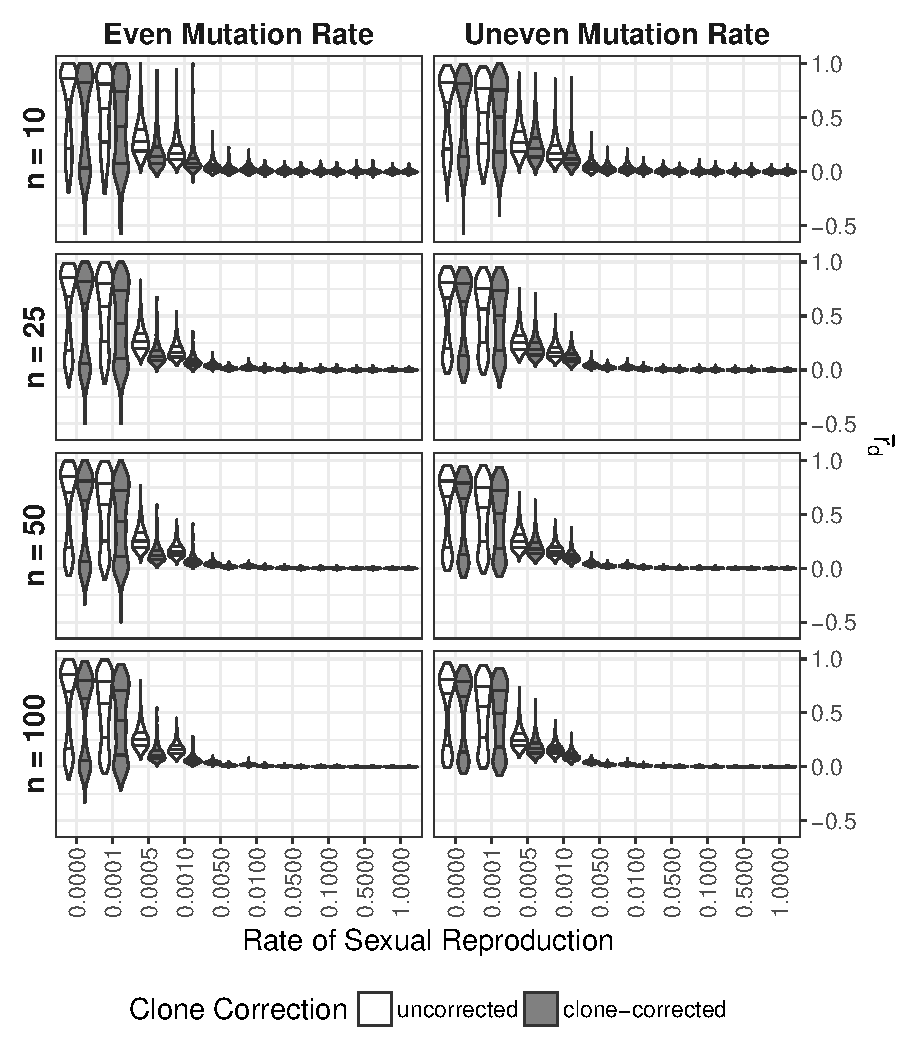
\includegraphics[width=1.00000\textwidth]{figure/rd_sexrate.pdf}
\caption{Effect of rate of sexual reproduction, sample size (n),
mutation rate, and clone-correction on \(\bar{r}_d\) for microsatellite
data. Violin plots represent data sets simulated with even and uneven
mutation rates over 20 and 21 loci, respectively (columns) and
sub-sampled in four different population sizes (rows). Color indicates
whether or not the calculations were performed on whole or
clone-corrected data sets. Each violin plot contains 1000 unique data
sets. Black lines in violins mark the 25, 50, and 75th
percentile.}\label{fig:sim1}
\end{figure}

\begin{figure}
\centering
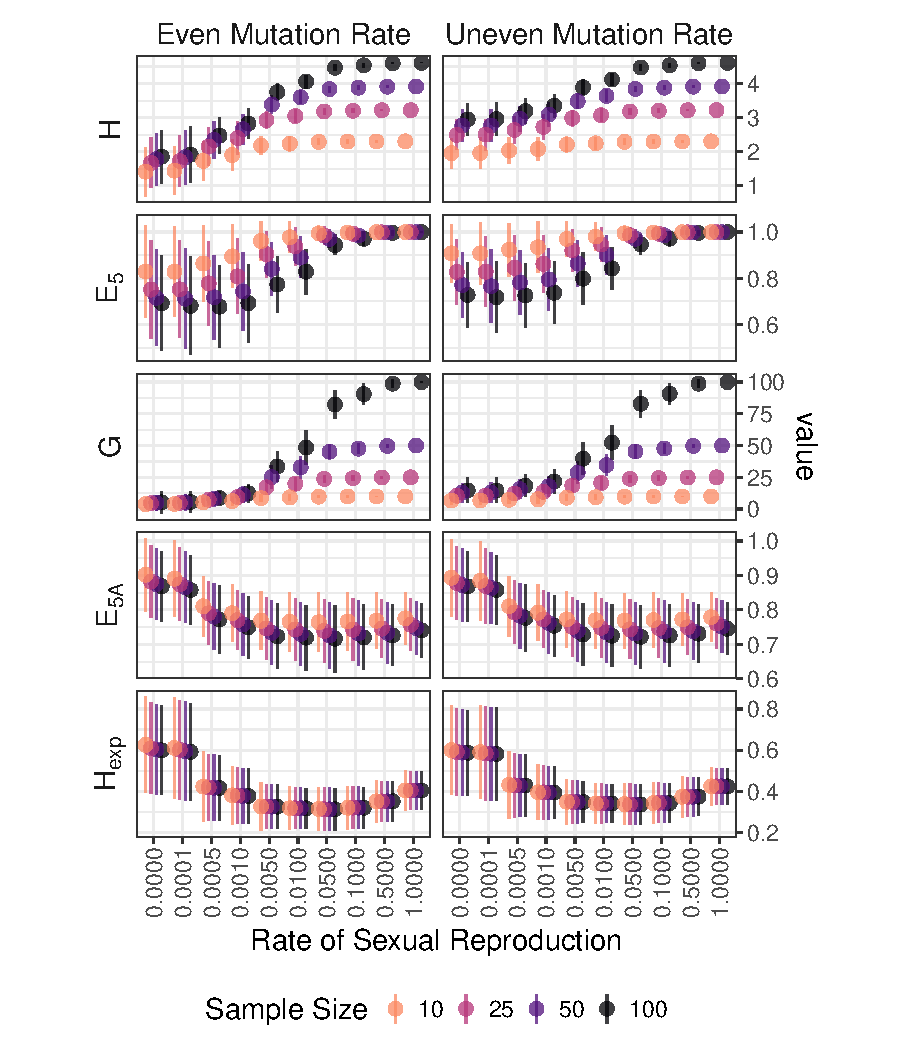
\includegraphics[width=1.00000\textwidth]{figure/diversity_stats.pdf}
\caption{Effect rate of sexual reproduction and sample size (n) on
genotypic and allelic diversity for microsatellite data. Genotypic
diversity: H = Shannon-Wiener index, \(E_5\) = evenness, G = Stoddart
and Taylor's index. Allelic Diversity: \(E_{5A}\) = allelic evenness,
\(H_{exp}\) = Nei's expected heterozygosity (gene diversity). Allelic
diversity estimates calculated for clone-corrected data. Points indicate
means and lines extend to to standard deviations on either side of the
mean. Color/shading indicates sample size. Vertical axis on different
scales.}\label{fig:simdiv}
\end{figure}

\begin{figure}
\centering
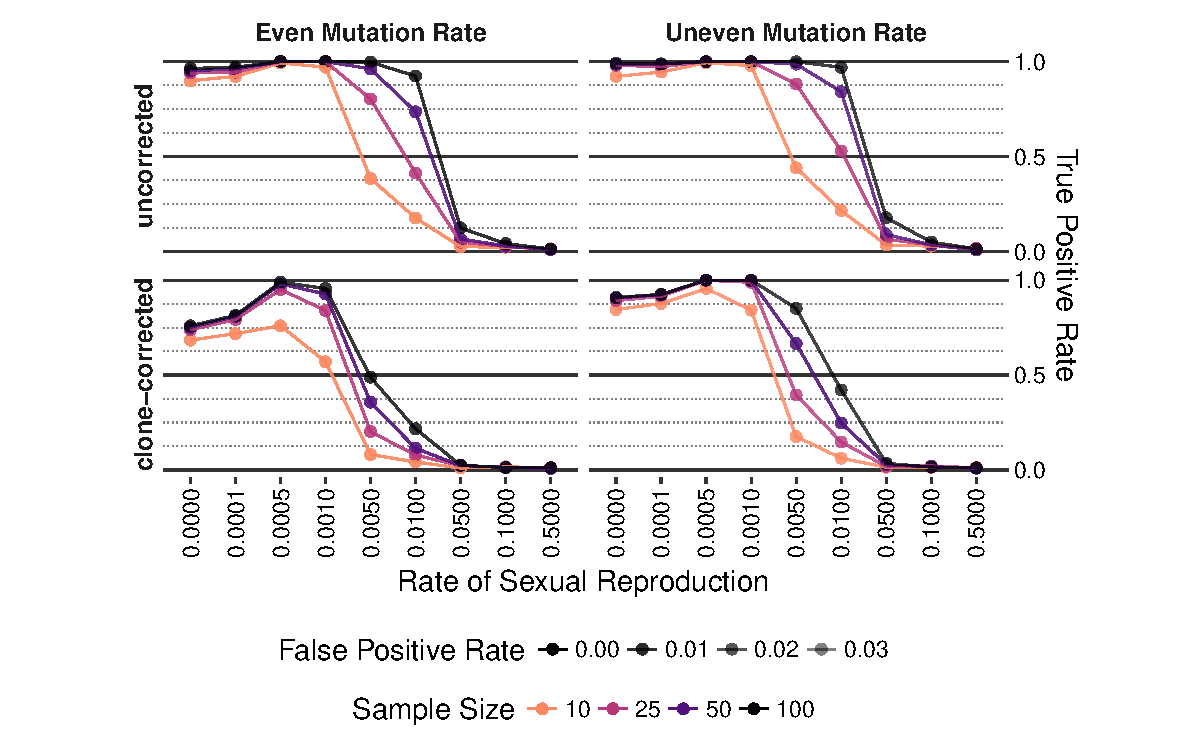
\includegraphics[width=1.00000\textwidth]{figure/ssr_power.pdf}
\caption{Effect of rate of sexual reproduction, sample size (n),
mutation rate, and clone-correction on the power of permutation analysis
for microsatellite data. Power (true positive rate) is on the vertical
axis. Values are shown for p = 0.01. Plots are arranged in a grid with
clone-correction in rows and mutation rate in columns. Color indicates
sample size.}\label{fig:sim4}
\end{figure}

\begin{figure}
\centering
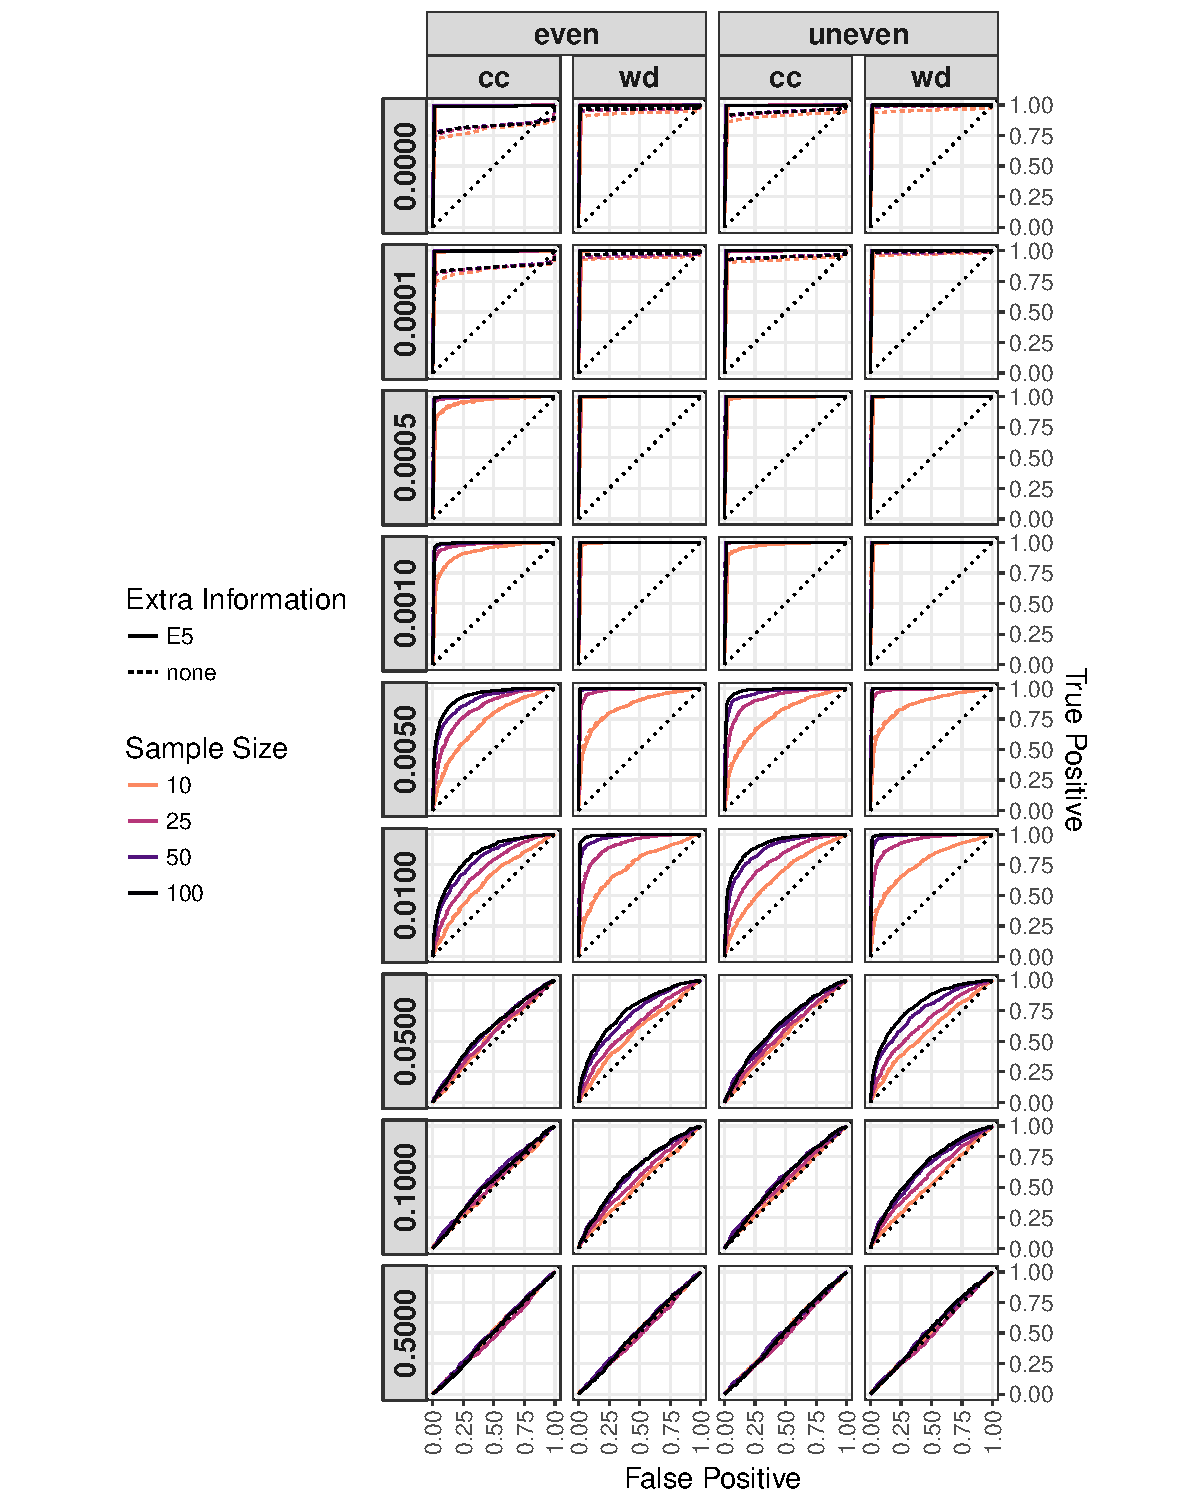
\includegraphics[width=1.00000\textwidth]{figure/ROC_Curve.pdf}
\caption{Effect of rate of sexual reproduction, sample size (n),
mutation rate, clone-correction, and \(E_{5A}\) augmentation on ROC
analysis of \(\bar{r}_d\). Rate of sexual reproduction arranged in rows.
Clone corrected (cc) and whole (wd) data sets with even and uneven
mutation rates arranged in columns. Line type indicates the use of
\(E_{5A}\) \textgreater{} 0.85 to augment the analysis. Line shade
indicates sample size. A dotted line of unity is shown in each plot.
Each ROC curve is calculated over 100 values of \(\alpha\) from 0 to
1.}\label{fig:simroc}
\end{figure}

\begin{figure}
\centering
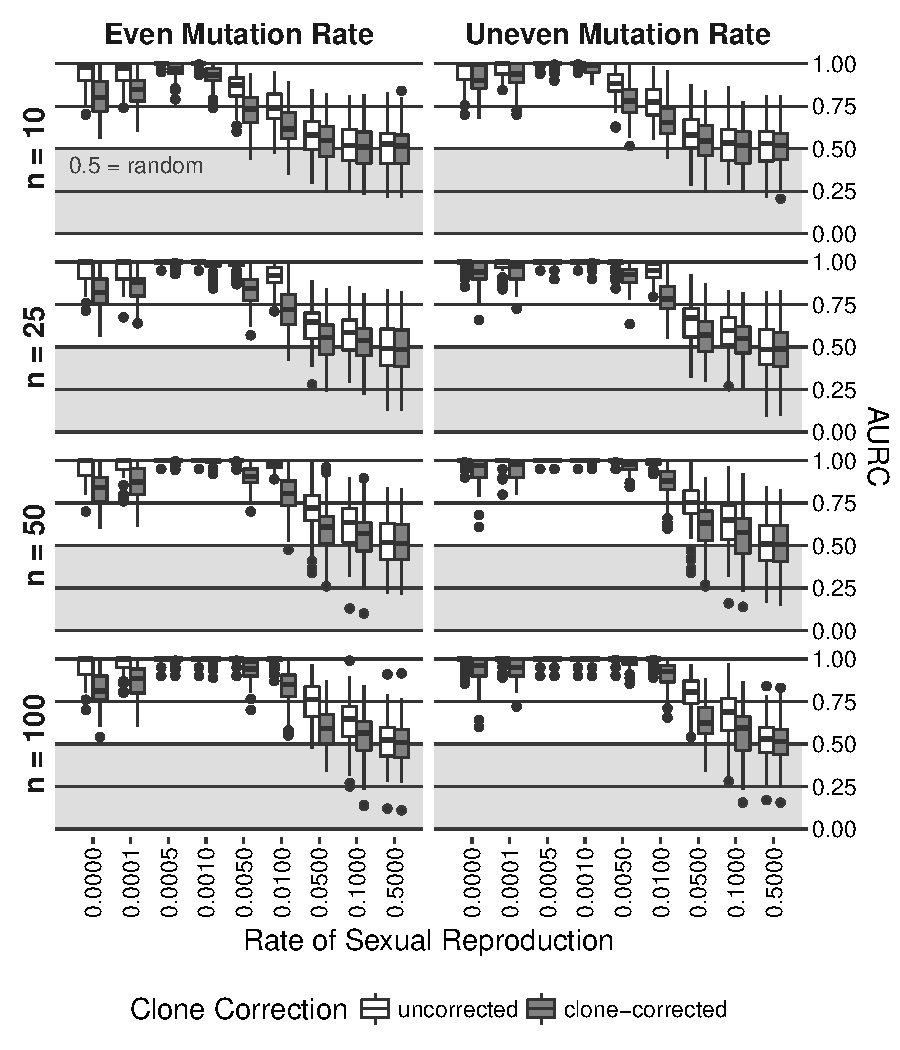
\includegraphics[width=1.00000\textwidth]{figure/AURC_box_plot.pdf}
\caption{Effect of rate of sexual reproduction, sample size (n),
mutation rate, and clone-correction on area under the ROC curve. Box
plots showing the distribution of the AURC for each independent seed.
Boxes span the interquartile range (IQR) and the whiskers extend to 1.5
* IQR. An AURC of 1 indicates a perfect classifier, while an AURC of 0.5
indicates the classifier is no better than a random guess. Any values
below 0.5 (shaded in grey) are considered worse than
random.}\label{fig:sim2}
\end{figure}

\begin{figure}
\centering
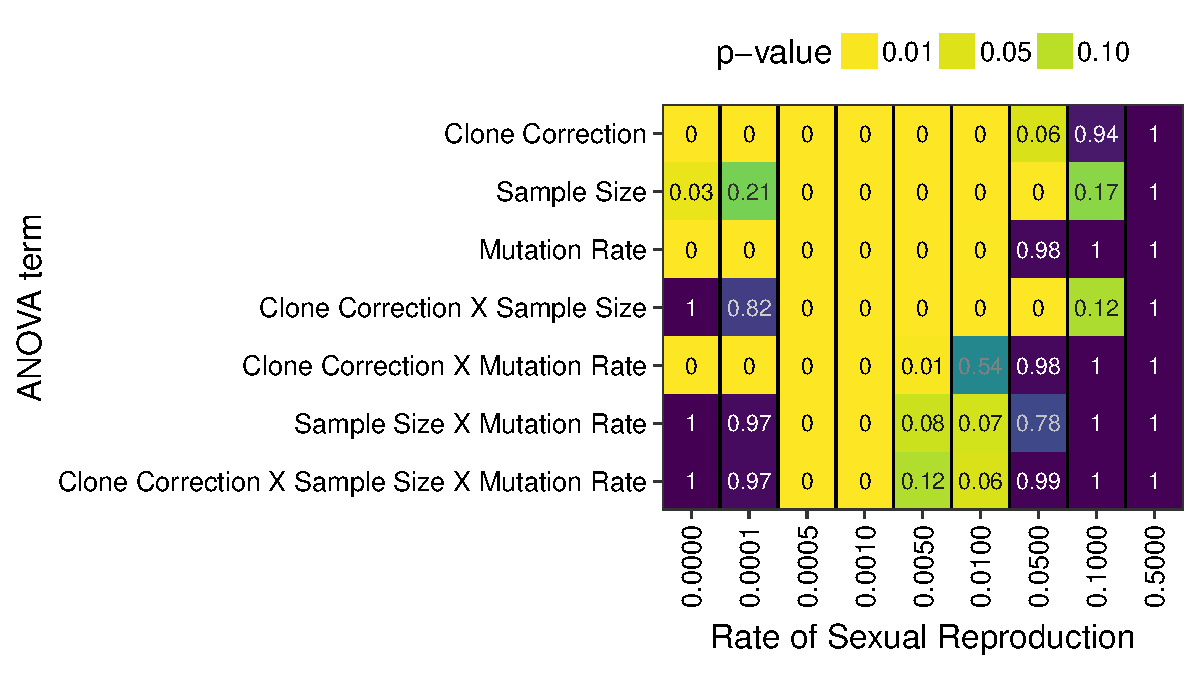
\includegraphics[width=1.00000\textwidth]{figure/AURC_ANOVA.pdf}
\caption{P-values from ANOVA analysis assessing AURC distributions with
the model
\(AURC \sim Clone Correction \times Sample Size \times Mutation Rate\)
for each rate of sexual reproduction, separately. P-values are
represented both as colors and numbers.}\label{fig:sim3}
\end{figure}

\begin{figure}
\centering
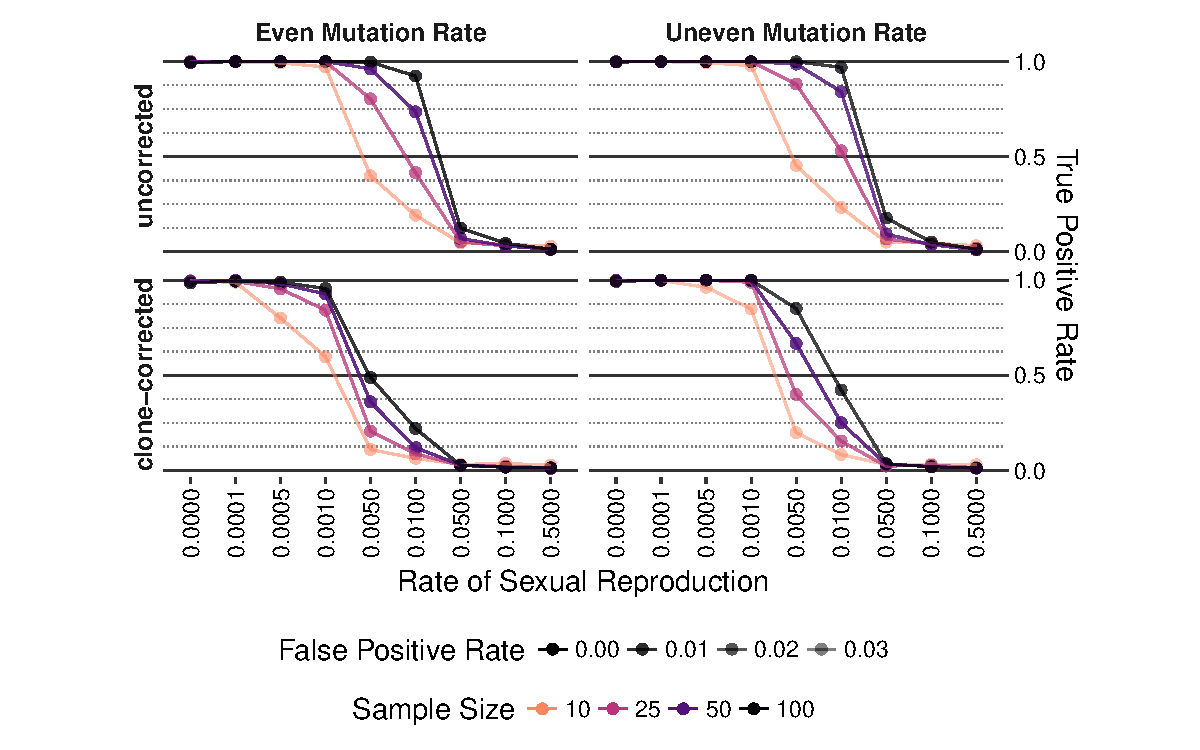
\includegraphics[width=1.00000\textwidth]{figure/ssr_power_ea.pdf}
\caption{Effect of rate of sexual reproduction, sample size (n),
mutation rate, and clone-correction on the power of permutation analysis
for microsatellite data taking into account allelic evenness. Plots are
arranged in a grid with clone-correction in rows and mutation rate in
columns. Values are shown for \(\alpha\) = 0.01 and
\(E_{5A} \geq 0.85\)}\label{fig:sim4a}
\end{figure}

\begin{figure}
\centering
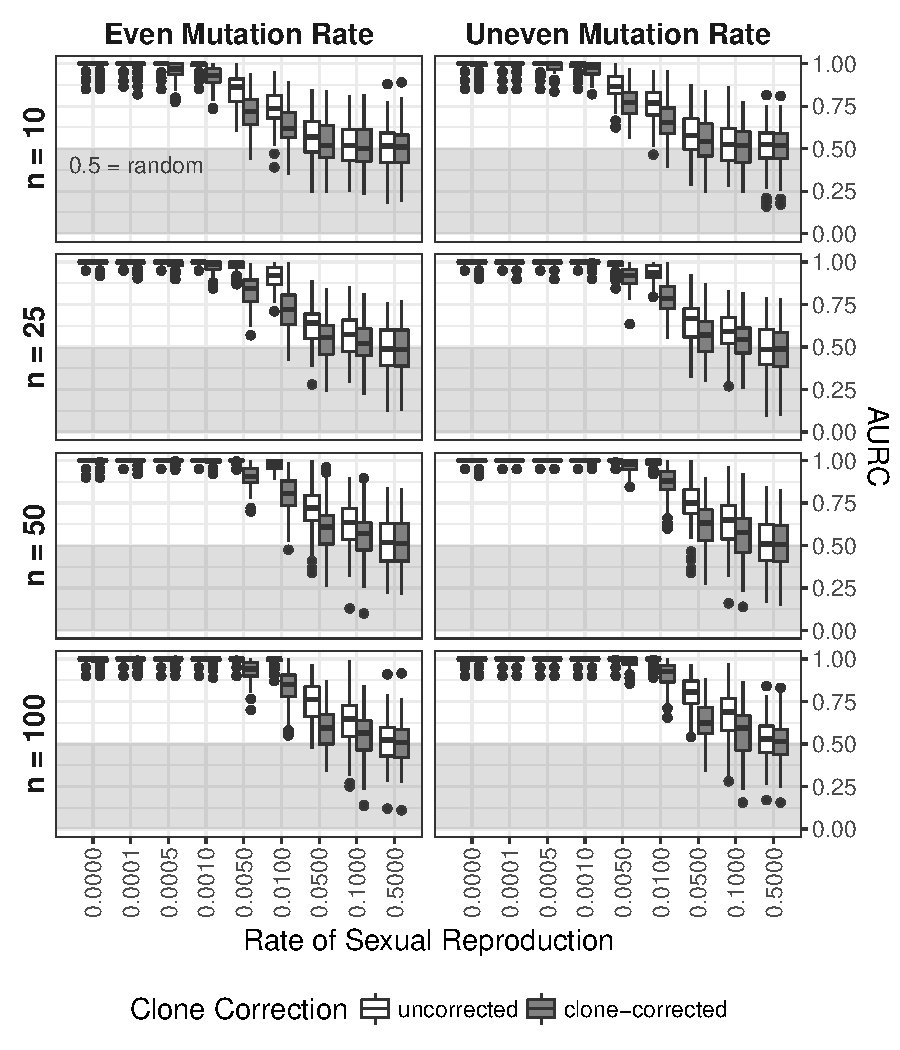
\includegraphics[width=1.00000\textwidth]{figure/AURC_box_plot_ea.pdf}
\caption{Effect of rate of sexual reproduction, sample size (n),
mutation rate, and clone-correction on area under the ROC curve taking
into account allelic evenness. Box plots showing the distribution of the
area under the ROC Curve for each independent seed. Boxes span the
interquartile range (IQR) and the whiskers extend to 1.5 * IQR. An AURC
of 1 indicates a perfect classifier, while an AURC of 0.5 indicates the
classifier is no better than a random guess. Any values below 0.5
(shaded in grey) is considered worse than random.}\label{fig:sim2a}
\end{figure}

\begin{figure}
\centering
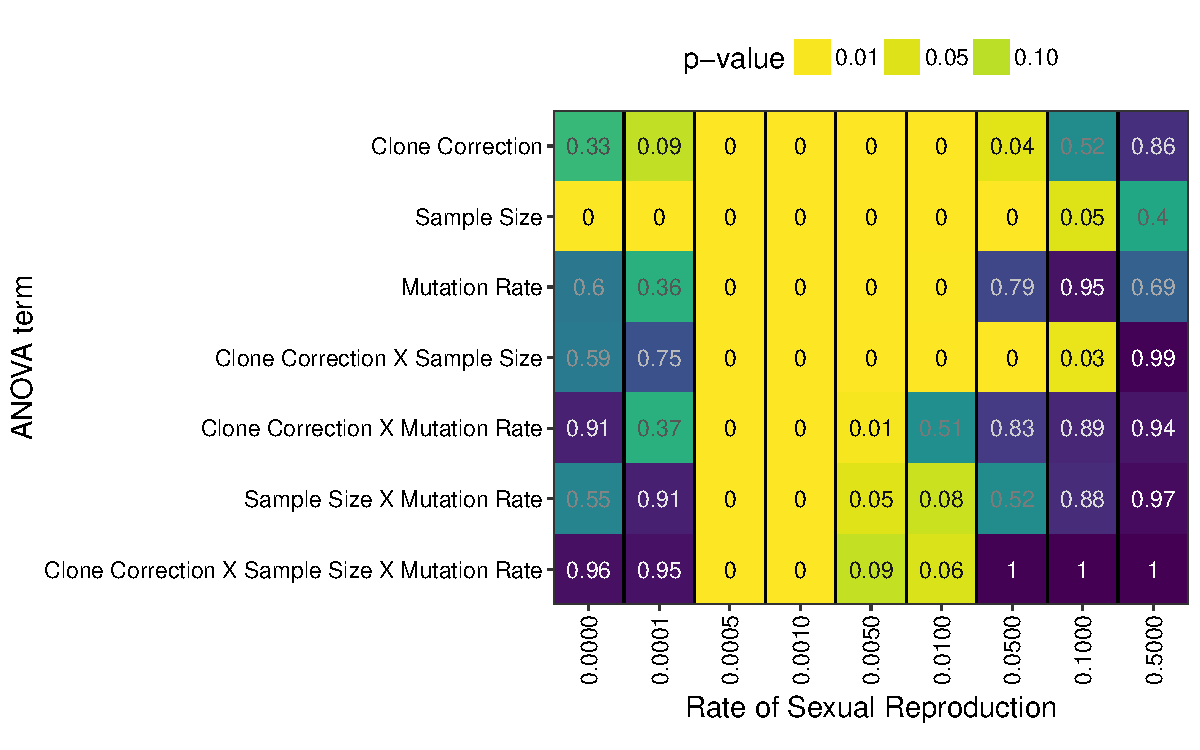
\includegraphics[width=1.00000\textwidth]{figure/AURC_ANOVA_ea.pdf}
\caption{P-values from ANOVA analysis on AURC distributions with the
model
\(AURC \sim Clone Correction \times Sample Size \times Mutation Rate\)
for each rate of sexual reproduction separately taking into account
allelic evenness. P-values are represented both as colors and
numbers.}\label{fig:sim3a}
\end{figure}

\begin{figure}
\centering
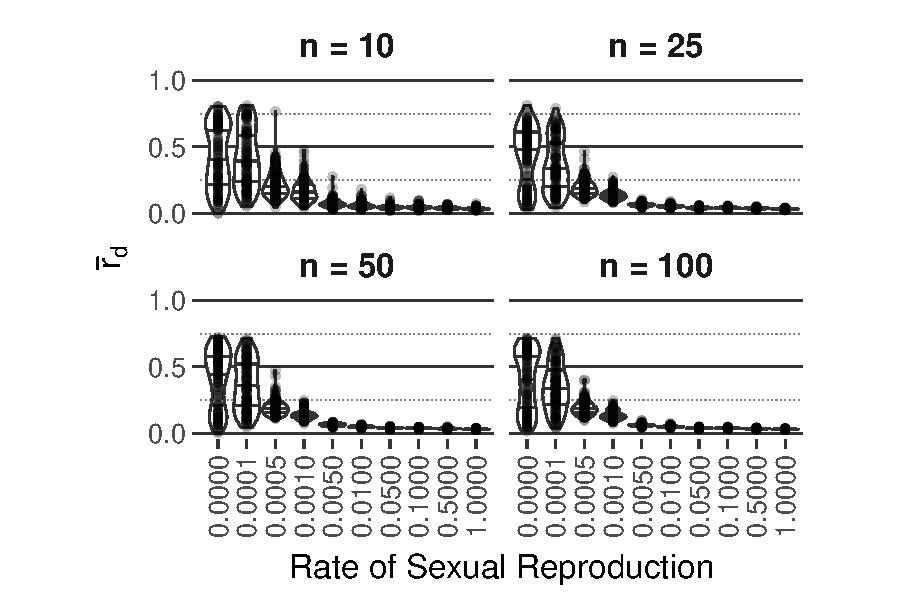
\includegraphics[width=1.00000\textwidth]{figure/genomic_rd.pdf}
\caption{Effect of rate of sexual reproduction and sample size (n) on
\(\bar{r}_d\) for SNP data. Each panel represents a different sample
size. Each violin plot contains 120 unique data sets. Points represent
observed values. Black lines in violins mark the 25, 50, and 75th
percentile.}\label{fig:sim5}
\end{figure}

\begin{figure}
\centering
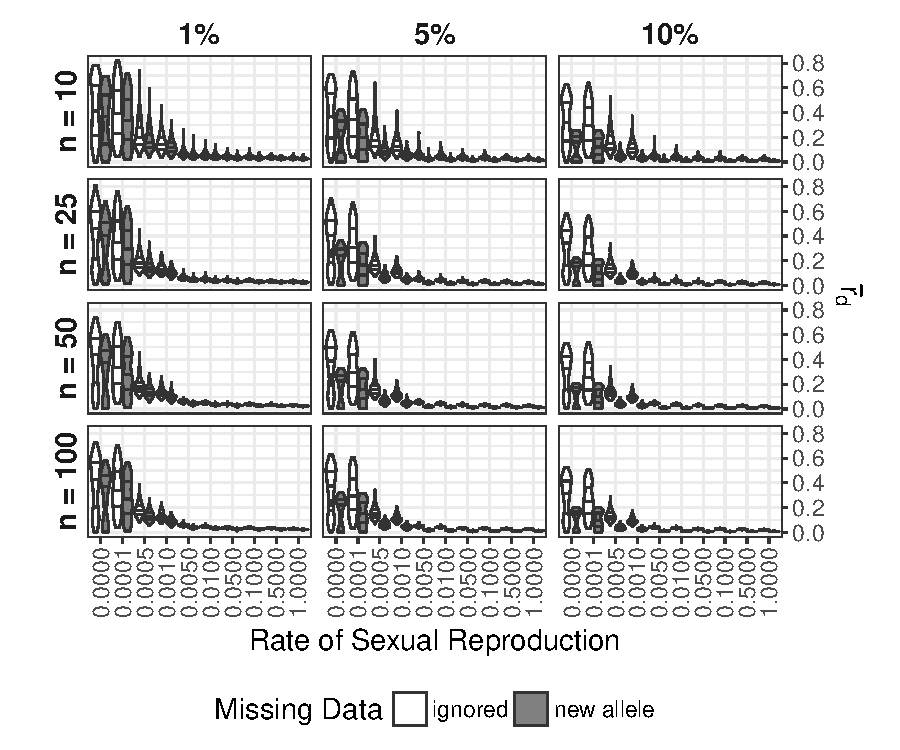
\includegraphics[width=1.00000\textwidth]{figure/genomic_missing.pdf}
\caption{Effect of rate of sexual reproduction, sample size (n), and
missing data on \(\bar{r}_d\) for SNP data. Panels are arranged
horizontally with increasing rates of missing data from left to right
and vertically with increasing sample size from top to bottom. Shading
indicates whether or not missing data was ignored or treated as a new
allele. Black lines mark the 25, 50, and 75th percentile. Each violin
represents 120 values.}\label{fig:simmisssnp}
\end{figure}

\begin{figure}
\centering
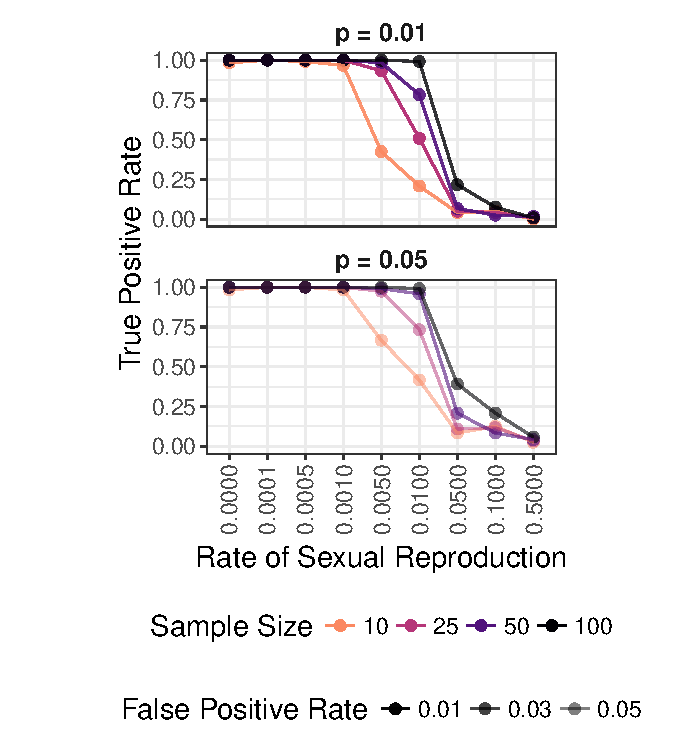
\includegraphics[width=1.00000\textwidth]{figure/genomic_power.pdf}
\caption{Effect of rate of sexual reproduction and sample size (n) the
power to detect non-random mating for SNP data. Color indicates sample
size. False positive rate is shown as increasing transparency. Data
shown for both p = 0.01 and p = 0.05}\label{fig:sim6}
\end{figure}

\begin{figure}
\centering
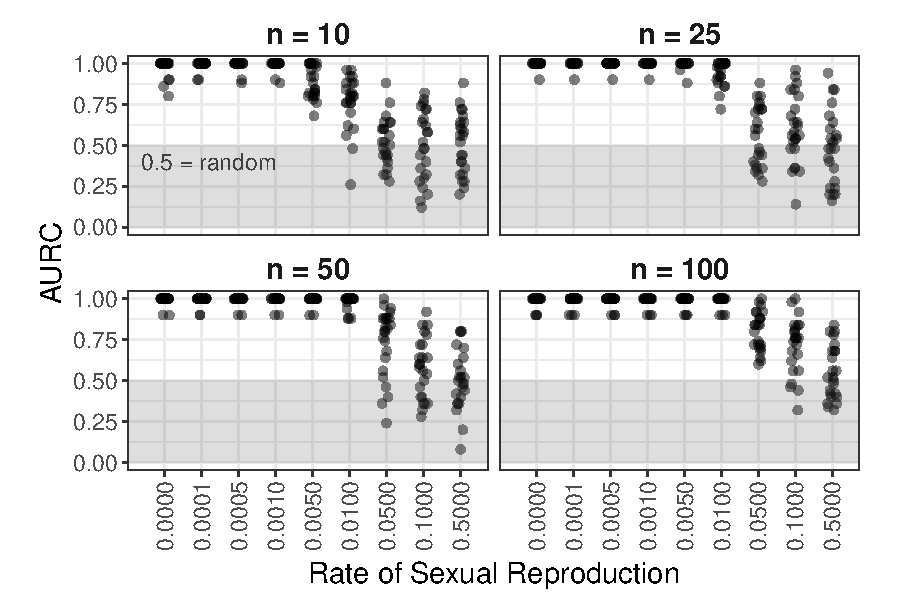
\includegraphics[width=1.00000\textwidth]{figure/AURC_genomic.pdf}
\caption{Effect of rate of sexual reproduction and sample size (n) on
area under the ROC curve for SNP data. Each point represents AURC
calculated with 10 populations total. 5 populations with a sex rate of
1.0 and 5 populations with a sex rate specified on the horizontal
axis.}\label{fig:sim7}
\end{figure}

\newpage

\subsection{Tables}\label{tables}

\begin{longtable}[]{@{}ccc@{}}
\caption{\label{tab:simtab1} Definitions of false positive and true positive
values for ROC analysis of simulations. \emph{p} is the p-value for
\(\bar{r}_d\), \(\alpha\) is a threshold value in {[}0, 1{]}. Randomly
mating populations are simulated with a sex rate of 1. Non-Random mating
populations are simulated with a sex rate less than one.}\tabularnewline
\toprule
Reproductive Mode & \(p \leq \alpha\) & \(p > \alpha\)\tabularnewline
\midrule
\endfirsthead
\toprule
Reproductive Mode & \(p \leq \alpha\) & \(p > \alpha\)\tabularnewline
\midrule
\endhead
Non-Random Mating & True Positive & False Negative\tabularnewline
Random Mating & False Positive & True Negative\tabularnewline
\bottomrule
\end{longtable}

\begin{longtable}[]{@{}llrrrr@{}}
\caption{\label{tab:sim3} ANOVA table comparing the model
\(AURC \sim Clone Correction \times Sample Size \times Mutation Rate\)
for each rate of sexual reproduction separately. Columns: sexrate = rate
of sexual reproduction, term = ANOVA term, sumsq = sum of squares, df =
degrees of freedom, statistic = F statistic, p.value = p-value, Terms
are as follows: CC = Clone Correction, SS = Sample Size, MR = Mutation
Rate.}\tabularnewline
\toprule
sexrate & term & sumsq & df & statistic & p.value\tabularnewline
\midrule
\endfirsthead
\toprule
sexrate & term & sumsq & df & statistic & p.value\tabularnewline
\midrule
\endhead
0.0000 & (Intercept) & 63.936 & 1 & 10569.674 & 0.000\tabularnewline
& CC & 0.855 & 1 & 141.309 & 0.000\tabularnewline
& SS & 0.060 & 3 & 3.289 & 0.020\tabularnewline
& MR & 0.556 & 1 & 91.913 & 0.000\tabularnewline
& CC X SS & 0.001 & 3 & 0.049 & 0.985\tabularnewline
& CC X MR & 0.174 & 1 & 28.747 & 0.000\tabularnewline
& SS X MR & 0.002 & 3 & 0.100 & 0.960\tabularnewline
& CC X SS X MR & 0.000 & 3 & 0.006 & 0.999\tabularnewline
& Residuals & 9.582 & 1584 & NA & NA\tabularnewline
0.0001 & (Intercept) & 70.972 & 1 & 14652.094 & 0.000\tabularnewline
& CC & 0.496 & 1 & 102.400 & 0.000\tabularnewline
& SS & 0.027 & 3 & 1.886 & 0.130\tabularnewline
& MR & 0.340 & 1 & 70.257 & 0.000\tabularnewline
& CC X SS & 0.009 & 3 & 0.596 & 0.617\tabularnewline
& CC X MR & 0.076 & 1 & 15.698 & 0.000\tabularnewline
& SS X MR & 0.001 & 3 & 0.077 & 0.972\tabularnewline
& CC X SS X MR & 0.003 & 3 & 0.241 & 0.868\tabularnewline
& Residuals & 7.673 & 1584 & NA & NA\tabularnewline
0.0005 & (Intercept) & 91.939 & 1 & 245382.751 & 0.000\tabularnewline
& CC & 0.072 & 1 & 191.181 & 0.000\tabularnewline
& SS & 0.089 & 3 & 78.753 & 0.000\tabularnewline
& MR & 0.050 & 1 & 132.414 & 0.000\tabularnewline
& CC X SS & 0.047 & 3 & 42.205 & 0.000\tabularnewline
& CC X MR & 0.027 & 1 & 72.663 & 0.000\tabularnewline
& SS X MR & 0.035 & 3 & 31.105 & 0.000\tabularnewline
& CC X SS X MR & 0.018 & 3 & 15.818 & 0.000\tabularnewline
& Residuals & 0.593 & 1584 & NA & NA\tabularnewline
0.0010 & (Intercept) & 86.202 & 1 & 157278.033 & 0.000\tabularnewline
& CC & 0.224 & 1 & 408.905 & 0.000\tabularnewline
& SS & 0.269 & 3 & 163.853 & 0.000\tabularnewline
& MR & 0.113 & 1 & 206.697 & 0.000\tabularnewline
& CC X SS & 0.135 & 3 & 82.053 & 0.000\tabularnewline
& CC X MR & 0.060 & 1 & 109.071 & 0.000\tabularnewline
& SS X MR & 0.067 & 3 & 40.994 & 0.000\tabularnewline
& CC X SS X MR & 0.034 & 3 & 20.426 & 0.000\tabularnewline
& Residuals & 0.868 & 1584 & NA & NA\tabularnewline
0.0050 & (Intercept) & 52.266 & 1 & 14127.572 & 0.000\tabularnewline
& CC & 0.936 & 1 & 253.111 & 0.000\tabularnewline
& SS & 2.592 & 3 & 233.531 & 0.000\tabularnewline
& MR & 0.138 & 1 & 37.393 & 0.000\tabularnewline
& CC X SS & 0.234 & 3 & 21.126 & 0.000\tabularnewline
& CC X MR & 0.028 & 1 & 7.675 & 0.006\tabularnewline
& SS X MR & 0.026 & 3 & 2.385 & 0.068\tabularnewline
& CC X SS X MR & 0.022 & 3 & 1.974 & 0.116\tabularnewline
& Residuals & 5.860 & 1584 & NA & NA\tabularnewline
0.0100 & (Intercept) & 39.376 & 1 & 5724.212 & 0.000\tabularnewline
& CC & 0.686 & 1 & 99.672 & 0.000\tabularnewline
& SS & 2.455 & 3 & 118.955 & 0.000\tabularnewline
& MR & 0.068 & 1 & 9.817 & 0.002\tabularnewline
& CC X SS & 0.173 & 3 & 8.380 & 0.000\tabularnewline
& CC X MR & 0.003 & 1 & 0.378 & 0.539\tabularnewline
& SS X MR & 0.051 & 3 & 2.488 & 0.059\tabularnewline
& CC X SS X MR & 0.056 & 3 & 2.720 & 0.043\tabularnewline
& Residuals & 10.896 & 1584 & NA & NA\tabularnewline
0.0500 & (Intercept) & 28.671 & 1 & 1903.303 & 0.000\tabularnewline
& CC & 0.072 & 1 & 4.806 & 0.029\tabularnewline
& SS & 0.239 & 3 & 5.293 & 0.001\tabularnewline
& MR & 0.001 & 1 & 0.080 & 0.778\tabularnewline
& CC X SS & 0.391 & 3 & 8.646 & 0.000\tabularnewline
& CC X MR & 0.000 & 1 & 0.032 & 0.858\tabularnewline
& SS X MR & 0.037 & 3 & 0.809 & 0.489\tabularnewline
& CC X SS X MR & 0.001 & 3 & 0.028 & 0.994\tabularnewline
& Residuals & 23.861 & 1584 & NA & NA\tabularnewline
0.1000 & (Intercept) & 26.010 & 1 & 1441.495 & 0.000\tabularnewline
& CC & 0.009 & 1 & 0.524 & 0.469\tabularnewline
& SS & 0.131 & 3 & 2.419 & 0.065\tabularnewline
& MR & 0.000 & 1 & 0.001 & 0.979\tabularnewline
& CC X SS & 0.162 & 3 & 2.984 & 0.030\tabularnewline
& CC X MR & 0.000 & 1 & 0.013 & 0.908\tabularnewline
& SS X MR & 0.014 & 3 & 0.256 & 0.857\tabularnewline
& CC X SS X MR & 0.001 & 3 & 0.015 & 0.998\tabularnewline
& Residuals & 28.581 & 1584 & NA & NA\tabularnewline
0.5000 & (Intercept) & 25.669 & 1 & 1489.342 & 0.000\tabularnewline
& CC & 0.001 & 1 & 0.033 & 0.857\tabularnewline
& SS & 0.042 & 3 & 0.806 & 0.491\tabularnewline
& MR & 0.002 & 1 & 0.099 & 0.753\tabularnewline
& CC X SS & 0.001 & 3 & 0.025 & 0.995\tabularnewline
& CC X MR & 0.000 & 1 & 0.006 & 0.939\tabularnewline
& SS X MR & 0.004 & 3 & 0.076 & 0.973\tabularnewline
& CC X SS X MR & 0.001 & 3 & 0.011 & 0.998\tabularnewline
& Residuals & 27.301 & 1584 & NA & NA\tabularnewline
\bottomrule
\end{longtable}

\begin{longtable}[]{@{}llrrrr@{}}
\caption{\label{tab:sim4} ANOVA table comparing the model
\(AURC \sim Clone Correction \times Sample Size \times Mutation Rate\)
for each rate of sexual reproduction separately. This table generated
with the allelic evenness correction. Columns: sexrate = rate of sexual
reproduction, term = ANOVA term, sumsq = sum of squares, df = degrees of
freedom, statistic = F statistic, p.value = p-value, Terms are as
follows: CC = Clone Correction, SS = Sample Size, MR = Mutation
Rate.}\tabularnewline
\toprule
sexrate & term & sumsq & df & statistic & p.value\tabularnewline
\midrule
\endfirsthead
\toprule
sexrate & term & sumsq & df & statistic & p.value\tabularnewline
\midrule
\endhead
0.0000 & (Intercept) & 96.914 & 1 & 169384.022 & 0.000\tabularnewline
& CC & 0.001 & 1 & 0.952 & 0.329\tabularnewline
& SS & 0.007 & 3 & 4.365 & 0.005\tabularnewline
& MR & 0.000 & 1 & 0.268 & 0.605\tabularnewline
& CC X SS & 0.001 & 3 & 0.638 & 0.591\tabularnewline
& CC X MR & 0.000 & 1 & 0.013 & 0.908\tabularnewline
& SS X MR & 0.001 & 3 & 0.704 & 0.550\tabularnewline
& CC X SS X MR & 0.000 & 3 & 0.104 & 0.958\tabularnewline
& Residuals & 0.906 & 1584 & NA & NA\tabularnewline
0.0001 & (Intercept) & 96.531 & 1 & 202595.988 & 0.000\tabularnewline
& CC & 0.001 & 1 & 2.838 & 0.092\tabularnewline
& SS & 0.009 & 3 & 6.345 & 0.000\tabularnewline
& MR & 0.000 & 1 & 0.823 & 0.365\tabularnewline
& CC X SS & 0.001 & 3 & 0.404 & 0.750\tabularnewline
& CC X MR & 0.000 & 1 & 0.819 & 0.366\tabularnewline
& SS X MR & 0.000 & 3 & 0.178 & 0.911\tabularnewline
& CC X SS X MR & 0.000 & 3 & 0.112 & 0.953\tabularnewline
& Residuals & 0.755 & 1584 & NA & NA\tabularnewline
0.0005 & (Intercept) & 91.136 & 1 & 158601.676 & 0.000\tabularnewline
& CC & 0.051 & 1 & 89.102 & 0.000\tabularnewline
& SS & 0.106 & 3 & 61.325 & 0.000\tabularnewline
& MR & 0.036 & 1 & 61.799 & 0.000\tabularnewline
& CC X SS & 0.033 & 3 & 19.237 & 0.000\tabularnewline
& CC X MR & 0.019 & 1 & 33.262 & 0.000\tabularnewline
& SS X MR & 0.024 & 3 & 14.139 & 0.000\tabularnewline
& CC X SS X MR & 0.012 & 3 & 7.046 & 0.000\tabularnewline
& Residuals & 0.910 & 1584 & NA & NA\tabularnewline
0.0010 & (Intercept) & 84.686 & 1 & 113261.634 & 0.000\tabularnewline
& CC & 0.211 & 1 & 282.532 & 0.000\tabularnewline
& SS & 0.339 & 3 & 151.115 & 0.000\tabularnewline
& MR & 0.103 & 1 & 137.833 & 0.000\tabularnewline
& CC X SS & 0.126 & 3 & 56.324 & 0.000\tabularnewline
& CC X MR & 0.053 & 1 & 71.367 & 0.000\tabularnewline
& SS X MR & 0.061 & 3 & 26.976 & 0.000\tabularnewline
& CC X SS X MR & 0.030 & 3 & 13.161 & 0.000\tabularnewline
& Residuals & 1.184 & 1584 & NA & NA\tabularnewline
0.0050 & (Intercept) & 51.087 & 1 & 13448.247 & 0.000\tabularnewline
& CC & 0.888 & 1 & 233.702 & 0.000\tabularnewline
& SS & 2.812 & 3 & 246.742 & 0.000\tabularnewline
& MR & 0.127 & 1 & 33.301 & 0.000\tabularnewline
& CC X SS & 0.226 & 3 & 19.851 & 0.000\tabularnewline
& CC X MR & 0.024 & 1 & 6.284 & 0.012\tabularnewline
& SS X MR & 0.031 & 3 & 2.682 & 0.045\tabularnewline
& CC X SS X MR & 0.025 & 3 & 2.186 & 0.088\tabularnewline
& Residuals & 6.017 & 1584 & NA & NA\tabularnewline
0.0100 & (Intercept) & 38.906 & 1 & 5499.579 & 0.000\tabularnewline
& CC & 0.634 & 1 & 89.610 & 0.000\tabularnewline
& SS & 2.558 & 3 & 120.521 & 0.000\tabularnewline
& MR & 0.070 & 1 & 9.912 & 0.002\tabularnewline
& CC X SS & 0.182 & 3 & 8.581 & 0.000\tabularnewline
& CC X MR & 0.003 & 1 & 0.443 & 0.506\tabularnewline
& SS X MR & 0.048 & 3 & 2.270 & 0.079\tabularnewline
& CC X SS X MR & 0.054 & 3 & 2.531 & 0.056\tabularnewline
& Residuals & 11.206 & 1584 & NA & NA\tabularnewline
0.0500 & (Intercept) & 28.404 & 1 & 1861.840 & 0.000\tabularnewline
& CC & 0.064 & 1 & 4.165 & 0.041\tabularnewline
& SS & 0.274 & 3 & 5.996 & 0.000\tabularnewline
& MR & 0.001 & 1 & 0.072 & 0.788\tabularnewline
& CC X SS & 0.401 & 3 & 8.760 & 0.000\tabularnewline
& CC X MR & 0.001 & 1 & 0.049 & 0.825\tabularnewline
& SS X MR & 0.035 & 3 & 0.759 & 0.517\tabularnewline
& CC X SS X MR & 0.001 & 3 & 0.020 & 0.996\tabularnewline
& Residuals & 24.165 & 1584 & NA & NA\tabularnewline
0.1000 & (Intercept) & 25.985 & 1 & 1413.238 & 0.000\tabularnewline
& CC & 0.008 & 1 & 0.422 & 0.516\tabularnewline
& SS & 0.145 & 3 & 2.632 & 0.049\tabularnewline
& MR & 0.000 & 1 & 0.004 & 0.952\tabularnewline
& CC X SS & 0.164 & 3 & 2.974 & 0.031\tabularnewline
& CC X MR & 0.000 & 1 & 0.019 & 0.891\tabularnewline
& SS X MR & 0.013 & 3 & 0.229 & 0.876\tabularnewline
& CC X SS X MR & 0.001 & 3 & 0.012 & 0.998\tabularnewline
& Residuals & 29.124 & 1584 & NA & NA\tabularnewline
0.5000 & (Intercept) & 25.366 & 1 & 1459.705 & 0.000\tabularnewline
& CC & 0.001 & 1 & 0.030 & 0.862\tabularnewline
& SS & 0.051 & 3 & 0.978 & 0.402\tabularnewline
& MR & 0.003 & 1 & 0.158 & 0.691\tabularnewline
& CC X SS & 0.001 & 3 & 0.026 & 0.994\tabularnewline
& CC X MR & 0.000 & 1 & 0.005 & 0.943\tabularnewline
& SS X MR & 0.004 & 3 & 0.078 & 0.972\tabularnewline
& CC X SS X MR & 0.001 & 3 & 0.010 & 0.999\tabularnewline
& Residuals & 27.526 & 1584 & NA & NA\tabularnewline
\bottomrule
\end{longtable}

\begin{longtable}[]{@{}llrrrr@{}}
\caption{\label{tab:sim5} ANOVA table comparing the model
\(AURC \sim Sample Size\) for each rate of sexual reproduction
separately with SNP data. Columns: sexrate = rate of sexual
reproduction, term = ANOVA term, sumsq = sum of squares, df = degrees of
freedom, statistic = F statistic, p.value = p-value, Terms are as
follows: SS = Sample Size.}\tabularnewline
\toprule
sexrate & term & sumsq & df & statistic & p.value\tabularnewline
\midrule
\endfirsthead
\toprule
sexrate & term & sumsq & df & statistic & p.value\tabularnewline
\midrule
\endhead
0.0000 & (Intercept) & 22.932 & 1 & 17347.604 & 0.000\tabularnewline
& sample & 0.004 & 3 & 1.121 & 0.345\tabularnewline
& Residuals & 0.122 & 92 & NA & NA\tabularnewline
0.0001 & (Intercept) & 23.602 & 1 & 29949.701 & 0.000\tabularnewline
& sample & 0.001 & 3 & 0.352 & 0.787\tabularnewline
& Residuals & 0.072 & 92 & NA & NA\tabularnewline
0.0005 & (Intercept) & 23.562 & 1 & 28317.512 & 0.000\tabularnewline
& sample & 0.001 & 3 & 0.339 & 0.797\tabularnewline
& Residuals & 0.077 & 92 & NA & NA\tabularnewline
0.0010 & (Intercept) & 23.562 & 1 & 28317.512 & 0.000\tabularnewline
& sample & 0.001 & 3 & 0.339 & 0.797\tabularnewline
& Residuals & 0.077 & 92 & NA & NA\tabularnewline
0.0050 & (Intercept) & 19.117 & 1 & 6103.399 & 0.000\tabularnewline
& sample & 0.174 & 3 & 18.568 & 0.000\tabularnewline
& Residuals & 0.288 & 92 & NA & NA\tabularnewline
0.0100 & (Intercept) & 13.984 & 1 & 1590.890 & 0.000\tabularnewline
& sample & 0.806 & 3 & 30.552 & 0.000\tabularnewline
& Residuals & 0.809 & 92 & NA & NA\tabularnewline
0.0500 & (Intercept) & 6.510 & 1 & 232.786 & 0.000\tabularnewline
& sample & 1.340 & 3 & 15.972 & 0.000\tabularnewline
& Residuals & 2.573 & 92 & NA & NA\tabularnewline
0.1000 & (Intercept) & 5.920 & 1 & 155.018 & 0.000\tabularnewline
& sample & 0.575 & 3 & 5.023 & 0.003\tabularnewline
& Residuals & 3.514 & 92 & NA & NA\tabularnewline
0.5000 & (Intercept) & 6.161 & 1 & 169.859 & 0.000\tabularnewline
& sample & 0.059 & 3 & 0.542 & 0.655\tabularnewline
& Residuals & 3.337 & 92 & NA & NA\tabularnewline
\bottomrule
\end{longtable}

\section*{References}\label{references}
\addcontentsline{toc}{section}{References}

\hypertarget{refs}{}
\hypertarget{ref-Agapow_2001}{}
Agapow P-M, Burt A (2001) Indices of multilocus linkage disequilibrium.
\emph{Molecular Ecology Notes}, \textbf{1}, 101--102.

\hypertarget{ref-ali2016cloncase}{}
Ali S, Soubeyrand S, Gladieux P \emph{et al.} (2016) Cloncase:
Estimation of sex frequency and effective population size by clonemate
resampling in partially clonal organisms. \emph{Molecular Ecology
Resources}.

\hypertarget{ref-arnaud2007standardizing}{}
Arnaud-Hanod S, Duarte CM, Alberto F, Serrão EA (2007) Standardizing
methods to address clonality in population studies. \emph{Molecular
Ecology}, \textbf{16}, 5115--5139.

\hypertarget{ref-arnaud2006genclone}{}
Arnaud-Haond S, Belkhir K (2006) Genclone: A computer program to analyse
genotypic data, test for clonality and describe spatial clonal
organization. \emph{Molecular Ecology Notes}, \textbf{7}, 15--17.

\hypertarget{ref-balloux2003population}{}
Balloux F, Lehmann L, de Meeûs T (2003) The population genetics of
clonal and partially clonal diploids. \emph{Genetics}, \textbf{164},
1635--1644.

\hypertarget{ref-brown1980multilocus}{}
Brown A, Feldman M, Nevo E (1980) Multilocus structure of natural
populations of \emph{Hordeum spontaneum}. \emph{Genetics}, \textbf{96},
523--536.

\hypertarget{ref-davey2010rad}{}
Davey JW, Blaxter ML (2010) RADSeq: next-generation population genetics.
\emph{Briefings in Functional Genomics}, \textbf{9}, 416--423.

\hypertarget{ref-davey2011genome}{}
Davey JW, Hohenlohe PA, Etter PD \emph{et al.} (2011) Genome-wide
genetic marker discovery and genotyping using next-generation
sequencing. \emph{Nature Reviews Genetics}, \textbf{12}, 499--510.

\hypertarget{ref-de2004clonal}{}
de Meeûs T, Balloux F (2004) Clonal reproduction and linkage
disequilibrium in diploids: A simulation study. \emph{Infection,
Genetics and Evolution}, \textbf{4}, 345--351.

\hypertarget{ref-de2006molecular}{}
de Meeûs T, Lehmann L, Balloux F (2006) Molecular epidemiology of clonal
diploids: A quick overview and a short DIY (do it yourself) notice.
\emph{Infection, Genetics and Evolution}, \textbf{6}, 163--170.

\hypertarget{ref-elshire2011robust}{}
Elshire RJ, Glaubitz JC, Sun Q \emph{et al.} (2011) A robust, simple
genotyping-by-sequencing (GBS) approach for high diversity species (L
Orban, Ed,). \emph{PLoS ONE}, \textbf{6}, e19379.

\hypertarget{ref-goss2014irish}{}
Goss EM, Tabima JF, Cooke DE \emph{et al.} (2014) The Irish potato
famine pathogen \emph{Phytophthora infestans} originated in central
Mexico rather than the Andes. \emph{Proceedings of the National Academy
of Sciences}, \textbf{111}, 8791--8796.

\hypertarget{ref-grunwald2003analysis}{}
Grünwald NJ, Goodwin SB, Milgroom MG, Fry WE (2003) Analysis of
genotypic diversity data for populations of microorganisms.
\emph{Phytopathology}, \textbf{93}, 738--746.

\hypertarget{ref-hartl1997principles}{}
Hartl DL, Clark AG (2007) \emph{Principles of population genetics}.
Sinauer Associates, Sunderland, MA, USA.

\hypertarget{ref-haubold1998detecting}{}
Haubold B, Travisano M, Rainey PB, Hudson RR (1998) Detecting linkage
disequilibrium in bacterial populations. \emph{Genetics}, \textbf{150},
1341--8.

\hypertarget{ref-heitman2012evolution}{}
Heitman J, Sun S, James TY (2012) Evolution of fungal sexual
reproduction. \emph{Mycologia}, \textbf{105}, 1--27.

\hypertarget{ref-jurasinski2014flux}{}
Jurasinski G, Koebsch F, Guenther A, Beetz S (2014) \emph{flux: Flux
rate calculation from dynamic closed chamber measurements}.

\hypertarget{ref-kamvar2015novel}{}
Kamvar ZN, Brooks JC, Grünwald NJ (2015a) Novel R tools for analysis of
genome-wide population genetic data with emphasis on clonality.
\emph{Frontiers in Genetics}, \textbf{6}.

\hypertarget{ref-kamvar2015poppr2supp}{}
Kamvar ZN, Brooks JC, Grünwald NJ (2015b) Supplementary Material for
Frontiers Plant Genetics and Genomics ``Novel R tools for analysis of
genome-wide population genetic data with emphasis on clonality''.

\hypertarget{ref-kamvar2015spatial}{}
Kamvar ZN, Larsen MM, Kanaskie AM, Hansen EM, Grünwald NJ (2015c)
Spatial and temporal analysis of populations of the sudden oak death
pathogen in oregon forests. \emph{Phytopathology}, \textbf{105},
982--989.

\hypertarget{ref-kamvar2014poppr}{}
Kamvar ZN, Tabima JF, Grünwald NJ (2014) Poppr : an R package for
genetic analysis of populations with clonal, partially clonal, and/or
sexual reproduction. \emph{PeerJ}, \textbf{2}, e281.

\hypertarget{ref-lynch2008genome}{}
Lynch M, Sung W, Morris K \emph{et al.} (2008) A genome-wide view of the
spectrum of spontaneous mutations in yeast. \emph{Proceedings of the
National Academy of Sciences}, \textbf{105}, 9272--9277.

\hypertarget{ref-mastretta2015restriction}{}
Mastretta-Yanes A, Arrigo N, Alvarez N \emph{et al.} (2014) Restriction
site-associated DNA sequencing, genotyping error estimation and \emph{de
novo} assembly optimization for population genetic inference.
\emph{Molecular Ecology Resources}, \textbf{15}, 28--41.

\hypertarget{ref-mcdonald1997population}{}
McDonald BA (1997) The population genetics of fungi: tools and
techniques. \emph{Phytopathology}, \textbf{87}, 448--453.

\hypertarget{ref-metz1978basic}{}
Metz CE (1978) Basic principles of ROC analysis. In: \emph{Seminars in
nuclear medicine}, pp. 283--298. Elsevier.

\hypertarget{ref-milgroom1996recombination}{}
Milgroom MG (1996) Recombination and the multilocus structure of fungal
populations. \emph{Annual Review of Phytopathology}, \textbf{34},
457--477.

\hypertarget{ref-milgroom2015population}{}
Milgroom MG (2015) \emph{Population biology of plant pathogens:
Genetics, ecology, and evolution}. APS Press, 3340 Pilot Knob Road, St.
Paul, MN 55121, USA.

\hypertarget{ref-Nei:1978}{}
Nei M (1978) Estimation of average heterozygosity and genetic distance
from a small number of individuals. \emph{Genetics}, \textbf{89},
583--590.

\hypertarget{ref-nielsen2013introduction}{}
Nielsen R, Slatkin M (2013) \emph{An introduction to population
genetics: Theory and applications}. Sinauer Associates, Incorporated.

\hypertarget{ref-nieuwenhuis2016frequency}{}
Nieuwenhuis BPS, James TY (2016) The frequency of sex in fungi.
\emph{Philosophical Transactions of the Royal Society B: Biological
Sciences}, \textbf{371}, 20150540.

\hypertarget{ref-orive1993effective}{}
Orive ME (1993) Effective population size in organisms with complex
life-histories. \emph{Theoretical Population Biology}, \textbf{44},
316--340.

\hypertarget{ref-peng2008forward}{}
Peng B, Amos CI (2008) Forward-time simulations of non-random mating
populations using simuPOP. \emph{Bioinformatics}, \textbf{24},
1408--1409.

\hypertarget{ref-pielou1975ecological}{}
Pielou E (1975) \emph{Ecological diversity}. Wiley \& Sons, New York.

\hypertarget{ref-prugnolle2010apparent}{}
Prugnolle F, de Meeûs T (2010) Apparent high recombination rates in
clonal parasitic organisms due to inappropriate sampling design.
\emph{Heredity}, \textbf{104}, 135--140.

\hypertarget{ref-R2016}{}
R Core Team (2016) \emph{R: A language and environment for statistical
computing}. R Foundation for Statistical Computing, Vienna, Austria.

\hypertarget{ref-rafiei2017comparison}{}
Rafiei V, Banihashemi Z, Jiménez-Díaz R \emph{et al.} Comparison of
genotyping by sequencing and microsatellite markers for unravelling
population structure in the clonal fungus \emph{Verticillium dahliae}.
\emph{Plant Pathology}.

\hypertarget{ref-shannon2001mathematical}{}
Shannon CE (1948) A mathematical theory of communication. \emph{ACM
SIGMOBILE Mobile Computing and Communications Review}, \textbf{5},
3--55.

\hypertarget{ref-smith1993how}{}
Smith JM, Smith NH, O'Rourke M, Spratt BG (1993) How clonal are
bacteria? \emph{Proceedings of the National Academy of Sciences},
\textbf{90}, 4384--4388.

\hypertarget{ref-stoddart1988genotypic}{}
Stoddart JA, Taylor JF (1988) Genotypic diversity: Estimation and
prediction in samples. \emph{Genetics}, \textbf{118}, 705--11.

\hypertarget{ref-taylor1999evolutionary}{}
Taylor JW, Geiser DM, Burt A, Koufopanou V (1999) The evolutionary
biology and population genetics underlying fungal strain typing.
\emph{Clinical Microbiology Reviews}, \textbf{12}, 126--146.

\hypertarget{ref-tibayrenc1996towards}{}
Tibayrenc M (1996) Towards a unified evolutionary genetics of
microorganisms. \emph{Annual Review of Microbiology}, \textbf{50},
401--429.


\end{document}
